%\documentclass[final,twocolumn,number,sort&compress]{elsarticle}
%\documentclass[review]{elsarticle}
%\documentclass[preprint,12pt,authoryear]{elsarticle}
%\documentclass[review,number,sort&compress]{elsarticle}
\documentclass[final,times,3p,twocolumn]{elsarticle}

\usepackage{lineno,hyperref}
%\usepackage{upgreek}
\usepackage{xcolor}
\usepackage{textcomp}

%\modulolinenumbers[5]

%\journal{Journal of \LaTeX\ Templates}

\linenumbers 
%\modulolinenumbers[5]

%\journal{Journal of \LaTeX\ Templates}

%%%%%%%%%%%%%%%%%%%%%%%
%% Elsevier bibliography styles
%%%%%%%%%%%%%%%%%%%%%%%
%% To change the style, put a % in front of the second line of the current style and
%% remove the % from the second line of the style you would like to use.
%%%%%%%%%%%%%%%%%%%%%%%

%% Numbered
%%\bibliographystyle{model1-num-names}

%% Numbered without titles
%\bibliographystyle{model1a-num-names}

%% Harvard
%\bibliographystyle{model2-names.bst}\biboptions{authoryear}

%% Vancouver numbered
%\usepackage{numcompress}\bibliographystyle{model3-num-names}

%% Vancouver name/year
%\usepackage{numcompress}\bibliographystyle{model4-names}\biboptions{authoryear}

%% APA style
%\bibliographystyle{model5-names}\biboptions{authoryear}

%% AMA style
%\usepackage{numcompress}\bibliographystyle{model6-num-names}

%% `Elsevier LaTeX' style
\bibliographystyle{elsarticle-num}
%%%%%%%%%%%%%%%%%%%%%%%
\journal{NIMA}

\begin{document}

\begin{frontmatter}
\title{Micromegas Vertex Tracker for CLAS12}

\author[A]{A. Acker} 
\author[A]{D. Atti\'e}
\author[A]{S. Aune}
\author[A]{J. Ball}
\author[A]{P. Baron}
\author[A]{Q. Bertrand}
\author[A]{D. Besin}
\author[A]{T. Bey}
\author[A]{F. Boss\`u}
\author[A]{R. Boudouin}
\author[A]{M. Boyer}
\author[A]{G. Charles}
\author[A]{G. Christiaens}
\author[A]{P. Contrepois}
\author[A]{M. Defurne}
\author[A]{E. Delagnes}
\author[A]{M. Garçon}
\author[A]{F. Georges}
\author[A]{R. Granelli}
\author[A]{N. Grouas}
\author[A]{C. Lahonde}
\author[A]{T. Lerch}
\author[A]{I. Mandjavidze}
\author[A]{O. Meunier}
\author[A]{Y. Mouden}
\author[A]{S. Procureur}
\author[A]{M. Riallot}
\author[A]{F. Sabati\'e}
\author[A]{E. Virique}
\author[A]{M. Vandenbroucke}



\address[A]{Irfu, CEA, Universit\'{e} Paris-Saclay, 91191, Gif-sur-Yvette, France}

\begin{abstract}

For the 12 GeV upgrade of Jefferson Laboratory, a Silicon Vertex Tracker (SVT) has been designed for the CLAS12 spectrometer using single-sided microstrip sensors fabricated by Hamamatsu. The sensors have a graded angle design to minimize dead areas and a readout pitch of 156 $\mu$m, with intermediate strips. Each double-sided SVT module hosts three daisy-chained sensors on each side with a full strip length of 33~cm. There are 512 channels per module, read out by four Fermilab Silicon Strip Readout (FSSR2) chips, featuring data-driven architecture, mounted on a rigid-flex hybrid board. The modules are assembled on the barrel using a unique cantilevered geometry to minimize the amount of material in the tracking volume. This paper is focused on the design, qualification of the performance, and experience in operating and commissioning the tracker during the first year of the data taking.

\end{abstract}

\end{frontmatter}

\section{Introduction}

This paper describes the software framework, tools, and algorithms that were developed in support of event
reconstruction and analysis of the CLAS12 (CEBAF Large Acceptance Spectrometer at 12 GeV) experiment at
Jefferson Lab (JLab)~\cite{clas12-nim}. Installed in experimental Hall~B, CLAS12 is a large acceptance
spectrometer based on two superconducting magnets and multiple detector subsystems that provides large
coverage for the detection of charged and neutral particles produced by the interaction of an electron beam
from the JLab CEBAF accelerator with a target located at the center of the spectrometer. A six-coil toroidal
magnet defines the six-sector structure of the so-called Forward Detector, including Drift Chambers~\cite{dc-nim}
for charged particle tracking, threshold Cherenkov Counters~\cite{ltcc-nim,htcc-nim} and Ring-Imaging Cherenkov
Counters~\cite{rich-nim} for particle identification, scintillator-based time-of-flight hodoscopes~\cite{ftof-nim},
and electromagnetic calorimeters~\cite{ecal-nim} based on a lead-scintillator sandwich design. In the target region,
a 5~T superconducting solenoid surrounds a central tracker based on silicon and Micromegas detectors
\cite{svt-nim,mm-nim}, a time-of-flight scintillation counter barrel~\cite{ctof-nim}, and a neutron detector
\cite{cnd-nim}, forming the so-called Central Detector. Figure~\ref{clas12-model} shows a model representation of
the CLAS12 spectrometer identifying the Forward and Central Detectors. In between the central and forward region,
the CLAS12 Forward Tagger~\cite{ft-nim} extends the kinematic coverage for the detection of electrons and photons
at polar angles from 2$^\circ$ to 5$^\circ$. Figure~\ref{ft-model} shows a model representation of the Forward
Tagger. The total number of readout channels of CLAS12 is larger than 100k, for a typical data rate in production
data taking of 400~MB/s (cross check with DAQ paper).  

\begin{figure}[t]
\centering
\includegraphics[width=0.48\textwidth]{pics/clas12-model.pdf}
\caption{Model representation of the CLAS12 spectrometer in Hall~B at Jefferson Laboratory. The electron
  beam is incident from the left side of this figure. The CLAS12 detector is roughly 20~m in scale along the
  beam axis. The CLAS12 Forward and Central Detectors are identified.}
\label{clas12-model}
\end{figure}

\begin{figure}
\centering
\includegraphics[width=0.48\textwidth]{pics/ft-model.pdf}
\caption{Model representation of the CLAS12 Forward Tagger that is positioned just upstream of the torus
  magnet along the beam axis. Attached to the upstream face of the detector is the M{\o}ller electron shielding
  cone.}
\label{ft-model}
\end{figure}

The CLAS12 offline reconstruction and analysis framework was developed to cope with the complexity of the
spectrometer and the related data volumes. It consists of an extensive library of software tools, of detector
reconstruction packages, and a framework to chain the reconstruction and analysis applications for data
processing. Software tools have been designed to support and standardize event reconstruction, detector
calibration and monitoring, and data analysis, providing I/O functionalities, database access, detector geometry
libraries, and magnetic field handling tools. These constitute the building blocks for the development of all CLAS12
detector monitoring, calibration, and reconstruction tools. Each reconstruction package is designed to extract
from the raw data the relevant information for particle reconstruction, such has tracks, hits, or clusters. These
are the input information for the CLAS12 Event Builder, which associates reconstructed detector output to
identify particles and form the reconstructed event. The reconstruction components are deployed in a
service-oriented platform, which provides the functionalities for data processing for both event reconstruction
and the subsequent analysis. While the software framework supports multiple programming languages, the CLAS12
reconstruction packages and tools currently in use are developed in Java.

This paper is organized as follows. The CLAS12 software framework and tools are described in
Section~\ref{sec:framework}. The raw and reconstructed data formats are presented in Section~\ref{sec-formats}.
The monitoring, calibration, and event display applications are described in Sections~\ref{sec:calibration} and
\ref{sec:ced}. Section~\ref{sec:recon} provides a detailed description of the detector and event reconstruction
packages, including selected results from reconstruction of simulated data that have been used to develop and
validate the algorithms. The reconstruction performance on beam data is presented in Ref.~\cite{clas12-nim}.
Finally, Sections~\ref{sec:dataproc} and \ref{sec:manage} present the data processing and code management
procedures adopted for CLAS12.

\section{Detector Layout}

\subsection{The Calorimeter (FT-Cal)}

The FT-Cal has to fulfill demanding requirements in terms of: radiation hardness, light yield, shower containment
(small radiation length and Moliere radius), fast recovery time, and good energy and time resolution.

The electron energy resolution is a crucial factor to determine precisely the photon energy and to ensure the
exclusivity of the measured reaction via the missing mass technique. However, since we are interested in low-energy
electrons and high-energy photons, the energy resolution on the latter is significantly better than the resolution on
the electron\footnote {For example, an electron energy resolution of 2\% (at 1~GeV) would result in an energy
  resolution of $\sim$0.2\% for the corresponding 10~GeV photon, allowing the use of the missing mass technique
  for most of the reactions of interest.}. The FT-Cal should have a fast recovery time ($\tau\sim$ 10~ns) to sustain
high rates with small pile-up effects and to provide the scattered electron interaction time with good accuracy
($<$1~ns) in order to reject background and to identify the relevant signals via coincidence with CLAS12. Due to the
expected high rate from electromagnetic background, the calorimeter should be highly segmented in the transverse
direction. The size of each detection element should be comparable with the characteristic transverse size of the
electromagnetic shower (Moliere radius) to contain the shower produced by incident electrons to a few readout cells,
thus minimizing rates and pile-up. Finally, the photodetectors for the light read out should work  in a sizable magnetic
field and fit within the available space. Thus, standard photomultipliers (PMTs) cannot be used while photodetectors
based on semiconductors, e.g. avalanche photodiodes (APDs), have been shown to meet the required criteria. 

To match the necessary requirements, lead tungstate (PbWO$_4$) was chosen as the scintillating material and
Large-Area APDs (LAAPDs) as the readout sensors. A similar  combination was used in the CMS-ECal~\cite{CMS-ECal},
CLAS-IC~\cite{CLAS-IC}, and PANDA-EMC~\cite{PANDA-ECal} calorimeters. Lead tungstate has a fast scintillation
decay time (6.5~ns), a small radiation length (0.9~cm), and small Moliere radius (2.1~cm). The drawback of limited
light emission (about 0.3\% of NaI(Tl)) has been mitigated by using cooled PbWO$_4$ Type-II crystals (as for the
PANDA-EMC), matched to large-area photosensors to obtain a factor of four more light per MeV of deposited energy
than the original CMS-ECal crystals.

With this design an energy resolution of the order of ($2\% /\sqrt{E\textrm{(GeV)}} \oplus 1\%$) is expected.
Other crystals, such as LSO/LYSO or the very recent LaBr, share almost all of the good specifications of
PbWO$_4$ with a light yield more than 100 times larger. However, the lack of extensive studies on radiation
hardness and the limited experience in the manufacturing procedures excluded them from consideration as an
alternative.

\begin{figure}[th!]
\centering 
\includegraphics[width=0.85\columnwidth]{fig/section.png} 
\caption{CAD drawing of the FT-Cal showing a cross section of the detector. The crystals, in purple, are enclosed in the copper thermal shield, in orange, surrounded by the insulation, in light gray. On the downstream end of the crystals (right side of the figure), the preamplifiers are shown in green. The weight of the crystals is supported by the tungsten pipe, in dark gray, which is an integral part of the beamline.}
\label{fig:ft-cal-geometry} 
\end{figure}

\subsubsection{Geometry and Coverage}

The FT-Cal is made from 332 $15\times 15\times 200$~cm$^3$ parallelepiped PbWO$_4$ Type-II crystals
arranged around the beamline with full azimuthal angular coverage ($0^\circ < \phi < 360^\circ$)  and small
forward angles acceptance ($2^\circ < \theta < 5^\circ$). The crystals are placed with their long side parallel to
the beamline to form a ring. Figure~\ref{fig:ft-cal-geometry} shows the a CAD rendering of the calorimeter. 

\subsubsection{PbWO$_4$ Crystals}

The FT-Cal PbWO$_4$ Type-II crystals were produced by the Shanghai Institute of Ceramics, Chinese Academy
(SICCAS). Since the light yield ($LY$) increases when lowering the temperature $T$ according to 
$dLY/dT \sim 3\%/^\circ$C, the calorimeter is stabilized in temperature and operated at
$T \sim 0^\circ$C. Lower temperatures were not considered due to significant complications in the
mechanical/thermal design, the reduced resistance to radiation,  and the decay time degradation of the cooled
PbWO$_4$. The length of the crystals (20~cm - corresponding to $\sim$22 radiation lengths) was chosen to
minimize the longitudinal loss and to match the available clearance.

The size of the crystal front face of 15~mm $\times$ 15~mm provides a pixelization in the transverse plane of
the PbWO$_4$ crystals consistent with the Moliere radius. All crystals were characterized using the ACCOS
(Automatic Crystal quality Control System) facility at CERN~\cite{accos}. The geometrical dimensions, as well as the
optical properties such as the longitudinal and transverse transmission and the relative light yield, were determined
for each of the crystals. Samples that were outside of the required specifications were rejected and replaced by the
manufacturer. 

The absolute $LY$ (number of detected photoelectrons per MeV deposited) was found to be $N_{pe}=220\pm 20$
at $T=0^\circ\textrm{C}\pm 0.5^\circ\textrm{C}$. For this measurement the crystal was wrapped on 5 of its faces
with 3M Vikuiti reflective film and read out by a Hamamatsu S8664-1010 LAAPD operated at a gain $G$=150
connected with optical grease on the exposed face. 

The scintillation decay time is also sensitive to the temperature. The time constant was measured using the
{\it Start-Stop} or {\it Delayed-Coincidence} method at different temperatures. As expected, an increase in the
decay constant was observed by decreasing the temperature. At $T=0^\circ\textrm{C}\pm 0.5^\circ\textrm{C}$, we
found $\tau=13.5\pm 0.6$~ns ($\tau_1=11.6\pm 0.5$~ns and $\tau_1=13.0\pm 0.2$~ns) when a single (double)
exponential form was used to fit the data.

\begin{figure}[th!]
\centering 
\includegraphics[width=0.85\columnwidth]{./fig/dk.jpeg} 
\caption{Histogram of the radiation-induced absorption coefficient, $dk$, for all SICCAS FT-Cal PbWO$_4$ crystals.}
\label{fig:dk} 
\end{figure}

The radiation hardness of the crystals was measured by irradiating them with a dose of 30~Gy of low-energy photons
using a $^{60}$Co source at the Strahlenzentrum of Giessen University~\cite{radhard}. The longitudinal transmission
was measured before and after the irradiation, calculating the variation as a function of the wavelength. The radiation
hardness of the crystals was quantified by the radiation-induced absorption coefficient defined as:

\begin{equation}
dk = \frac{1}{L}\frac{T_{bef}}{T_{irr},}
\end{equation}

\noindent
where $T_{bef}$ is the light transmission at 420~nm, the peak of the PbWO$_4$ emission spectrum, measured before
irradiation, and $T_{irr}$ is the light transmission at the same wavelength after irradiation for crystals of a given
length $L$. Crystals exhibiting greater levels of radiation damage to light transmission have higher values of $dk$.
All 332 crystals assembled in the FT-Cal were individually characterized: on average we found 
$T_{bef}$(420~nm) = $61.5 \pm 0.2$ ($\sigma=3.2$) and $T_{irr}$(420~nm) = $50.8 \pm 0.5$ ($\sigma=4.9$). 
The resulting $dk$ distribution is shown in Fig.~\ref{fig:dk}. These measurements were used to optimize the position
of each crystal in the calorimeter, placing the crystals with the highest radiation resistance, and therefore lowest
$dk$, in the areas where the highest radiation dose is expected.

\begin{figure}[th!]
\centering 
\includegraphics[width=1.0\columnwidth]{./fig/apd5.eps} 
\caption{Intrinsic gain of one APD as a function of the bias voltage and of the temperature.}
\label{fig:G-V-T} 
\end{figure}

\subsubsection{Light Readout and Electronics}
\label{sec:ftcalread}

The FT-Cal uses $10 \times 10$~mm$^2$ (model Hamamatsu S8664-1010) LAAPDs to read out the PbWO$_4$
scintillation light. APDs are very compact devices (only a few mm thick), have a large quantum efficiency at the
PbWO$_4$ light peak emission (420~nm), and  are insensitive to magnetic fields. The main disadvantage is that,
due to their low intrinsic gain ($\sim$50-200), the output signal is too small to be directly acquired, and needs to
be amplified by a suitable circuit. APDs also need to be operated at a controlled temperature to avoid variations in
gain and noise, but this does not represent a major complication since the crystals also are required to be stabilized
in temperature. Each sensor used in the FT-Cal has been characterized by measuring its gain as a function of the
applied bias voltage at a given temperature using an automated  custom facility (see Ref.~\cite{celeAPD} for more
details). The typical gain behavior $G(V_{Bias},T)$ is shown in Fig.~\ref{fig:G-V-T}. The working point (bias voltage)
was chosen in order to have the chosen gain ($G=150$) in a reasonably stable region for small variation of the biasing.
Silicon photomultiplier (SiPM) readout was not considered due to their limited dynamic range, which is not suitable for
spectroscopic applications, and the limited experience (in term of reliability, radiation hardness, stability in time, etc.)
in their use in large experiments at this time.

The APD current signal is converted to a voltage pulse that is transmitted to the subsequent electronics chain via a
trans-impedance amplifier (i.e. an amplifier that converts an input current pulse into an output voltage pulse, without
performing any time integration). This amplifier has been developed in collaboration with the Service Electronique
pour la Physique (SEP) of the Institut de Physique Nucl{\'e}aire (IPN) in Orsay. The amplifier ENC \footnote{The ENC,
  equivalent noise charge, is defined as the charge transported by an input signal giving, at the output of the amplifier,
  a signal whose amplitude is equal to the RMS of the output noise.} was measured at the operating temperature of
T=0$^\circ$C,  with ENC$\sim10400$ $e^-$ (RMS) for the nominal gain of $G=600$.  This corresponds to about 3 MeV (RMS) on the measured energy. The amplified signal is read out using the custom JLab flash
ADC VME board (a 16-channel, 12-bit, 250~MHz digitizer; referred to as the FADC250). The measurement
of the full waveform allows for the derivation of both the charge and time of the hit with the required  accuracy.

\subsubsection{Light Monitoring System}

Lead tungstate scintillating crystals are known as an appropriate material for use in total absorption shower
detectors. Unfortunately, although relatively radiation tolerant, their light output is reduced when exposed to 
radiation and recovers when the radiation source is removed. Further complications arise because at the same
irradiation intensity, changes in light output may vary from one crystal to another. In order to maintain the intrinsic
energy resolution, the crystals have to be continuously monitored and, if necessary, re-calibrated by changing the
supply voltage. The monitoring system should be able to test the response over time of the whole chain: crystal,
APD, read-out electronics. Among the different possible options (radioactive source, laser, and LED) we used an
LED-based Light Monitoring System (LMS). In spite of the need for thermal control, LEDs offer considerable
advantages: matching with crystals is simpler than for lasers, since each crystal can have a LED in front of it and
the arrangement of power lines and electrical connections is less critical than for optical fibers. The main
disadvantage is related to the complexity of the electronic circuitry: to cover a large light intensity range while
maintaining a good timing, each LED needs a separate driver, which leads for a calorimeter of significant size, to
a large number of electronic circuits.

With LEDs it is possible to obtain a shape and a duration of the monitoring-light flash that is similar to the features
of the crystal scintillation light. In fact, the emission spectrum of the monitoring light can be chosen to be similar to
the radio-luminescence spectrum of PbWO$_4$, the effective optical path length for monitoring light in the crystal
can be matched to the average path length of the scintillation light produced by an electromagnetic shower, and the
pulse length can be tuned to reproduce the PbWO$_4$ scintillation decay time. We chose a blue light LED with
wavelength close to the 430~nm emission peak of the PbWO$_4$ crystal, where radiation damage may have the
maximum effect. Each crystal is equipped with a separate LED, located on its upstream face, at the
opposite end with respect to the light sensors and electronics. The intensity can be varied in the range from 500 to
100,000 photons, pulsed at a variable rate from 62~Hz to 8~kHz, with a pulse rise time of $\sim$1~ns and a time
jitter of less than 200~ps. The system has been designed to work in the temperature range from -25$^\circ$C
to +30 $^\circ$C. The LEDs placed in the closed environment of the crystal are kept at constant temperature with an
accuracy of $\Delta T$ = 0.1$^\circ$C. The LED monitoring system is split in two boards: one containing the control
logic and the LED driver circuits, and the other, mounted in front of the FT-Cal crystals, hosting the LEDs. The two
boards are connected via a board-to-board connector that allows the required flexibility to match the FT-Cal
geometry and positioning. The LED drivers are controlled by an on-board PIC32 micro-controller accessible remotely
via Ethernet. Each LED is individually set by a programmable length and intensity pulse. The system is triggered by
an internal clock or by an external signal. In both cases the trigger signal is available for a precise time reference. 

\begin{figure}[th!]
\centering 
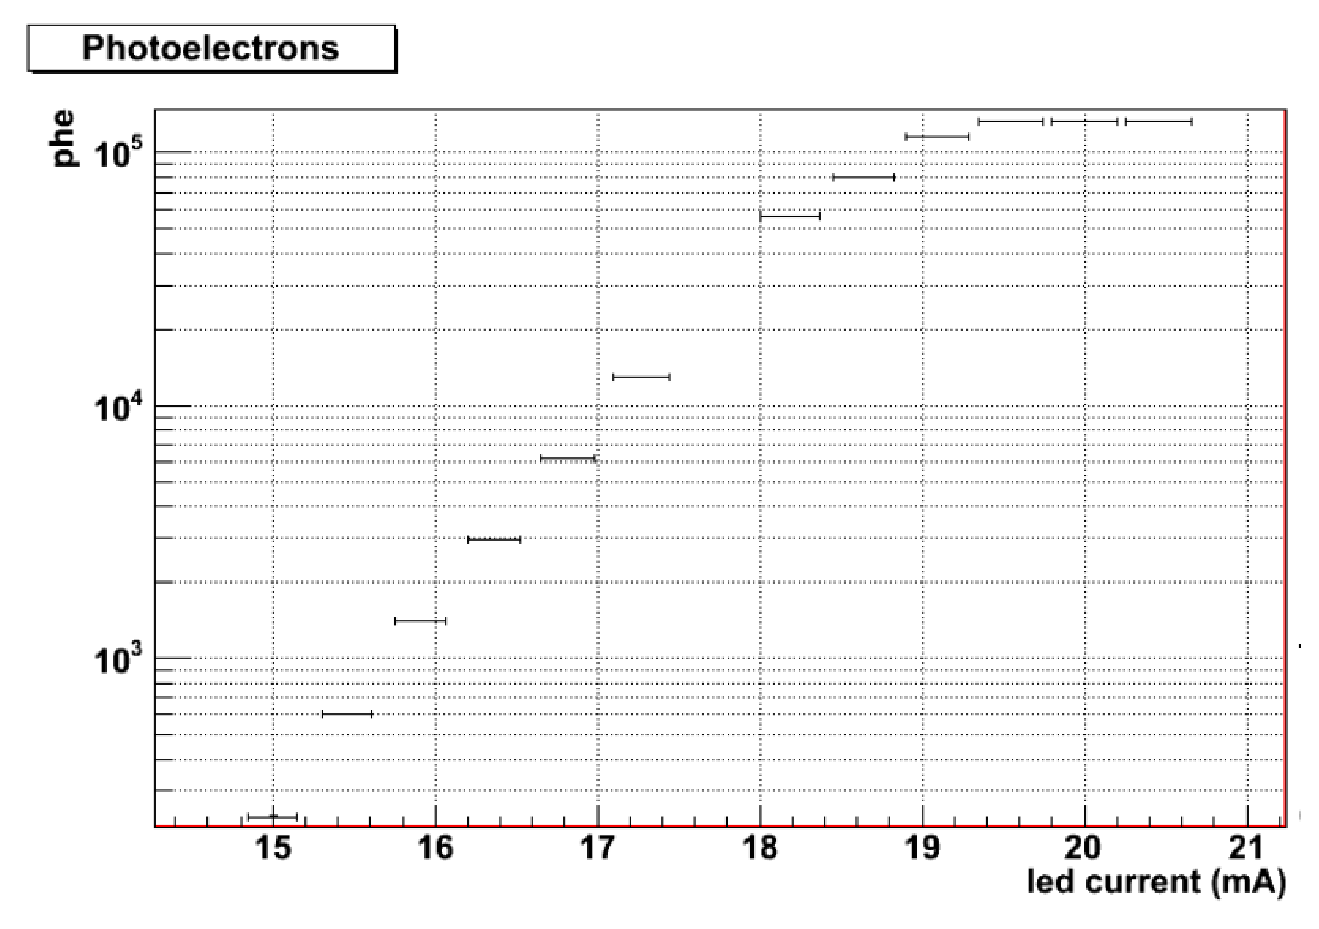
\includegraphics[width=1.0\columnwidth]{./fig/dynamics.eps}
\caption{Number of photoelectrons as a function of the LED driver current. The corresponding energy per crystal
  ranges from 10~MeV to 10~GeV.}
\label{fig:LEDperf1} 
\end{figure}

\begin{figure}[th!]
\centering 
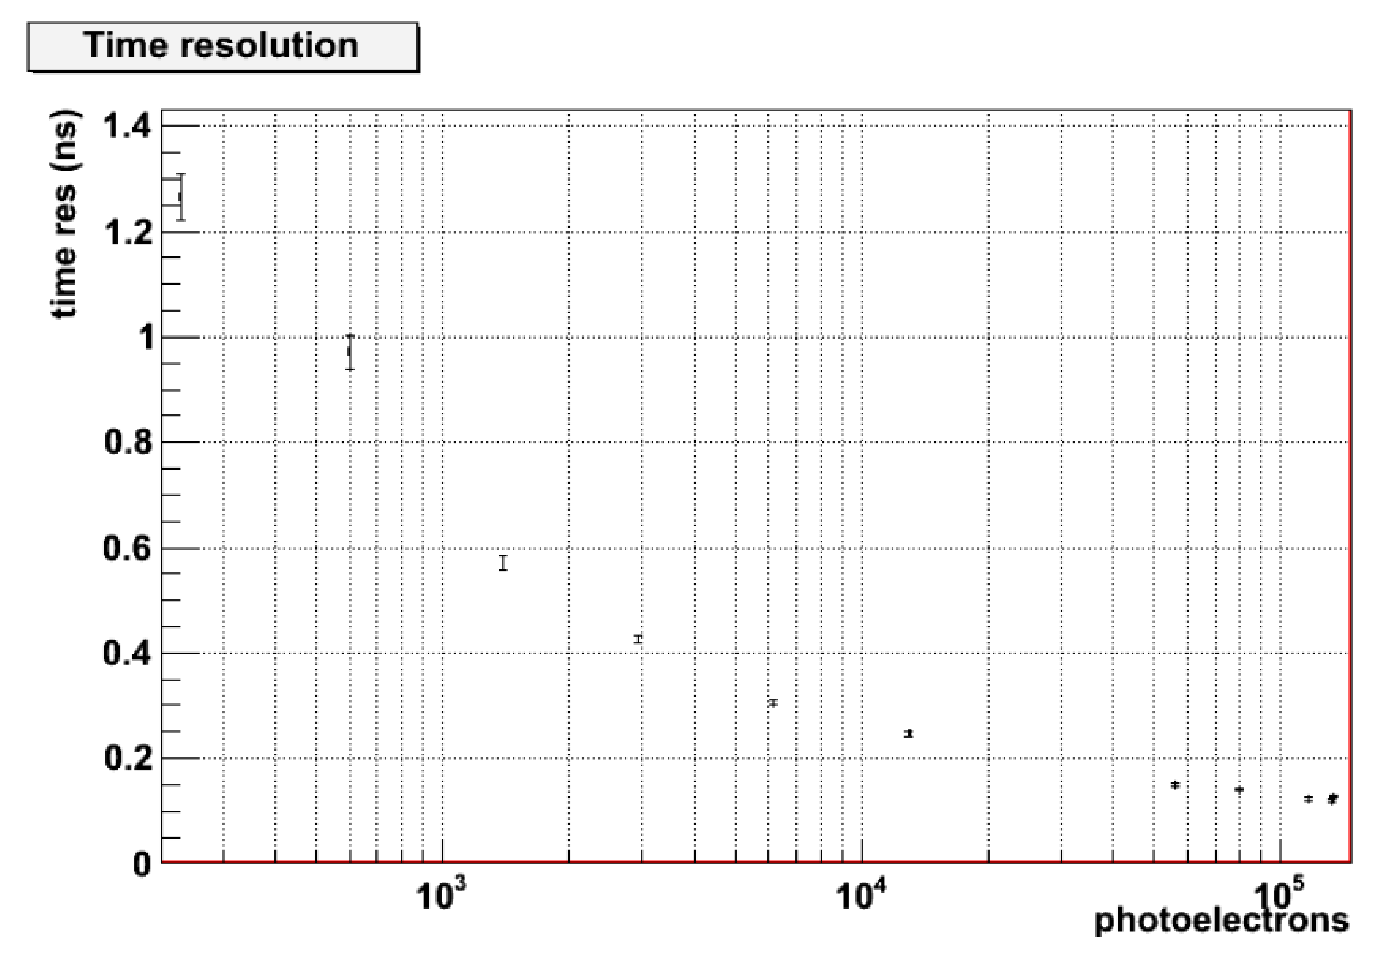
\includegraphics[width=1.0\columnwidth]{./fig/timing.eps}
\caption{Time resolution (measured as the time difference of the trigger signal and the PMT pulse) as a function of
  the LED light intensity.}
\label{fig:LEDperf2} 
\end{figure}

The performance of the LED driver has been measured by coupling a single monitoring channel to a PMT. The
performance of the system is reported in Figs.~\ref{fig:LEDperf1} and \ref{fig:LEDperf2}, where the measured
number of photoelectrons as a function of the LED current and the measured time resolution as a function of the
number of photoelectrons are shown\footnote{The time resolution is defined as the width ($\sigma$) of the time
  difference distribution between the trigger signal and the PMT output.}. Rescaling the results to take into account
the APD readout and the crystal $LY$/MeV, the equivalent energy ranges from 10~MeV (500~phe) to 10~GeV
(500k~phe) perfectly matched to the expected energy collected by each crystal. A time resolution of 100~ps is
reached at high light intensity. The long term stability of the system has been measured over a 100-hr run at
$T=+18^\circ$C. The stability of each individual channel was found to be in the range of 2\%; when the ratio of
the two channels is considered, the stability is at a level of a few parts per thousand.

\subsubsection{Slow Controls and Interlocks}

The FT-Cal slow controls are part of the CLAS12 EPICS system~\cite{daq}. The APDs need to be reverse-biased
with a positive high-voltage power source. The APD intrinsic gain depends on the bias voltage with
$\frac{1}{G}\frac{\Delta G}{\Delta V} \sim4 \%$ and, therefore, the power supply needs to be stable in time, with
low output noise. We chose the CAEN A1520P board designed for the CMS electromagnetic calorimeter. The power
supply fulfills  all our requirements in terms of dynamic range, linearity, and noise. Each board is equipped with 12
independent channels that each control a group of ten APDs with relative gain variations not greater than 3\%.

The amplifiers used in the FT-Cal need to be operated with +5~V and -5~V. The power consumption from each of the
two voltage sources is approximately 70~mW, almost independent of the event rate, giving a power consumption of
$\sim$140~mW per board, for a total of 56~W for a 400-channel calorimeter. The full FT-Cal is powered by a
Wiener MPOD MPV8008L power supply. Sensing feedback is implemented to compensate the voltage drop across the
connecting cables.

Temperature regulation is provided by a Lauda XT150 chiller unit. This is a self-regulating unit and does not require
external feedback, however, the settings and monitored parameters are sent to EPICS for recording via a
{\it streamDevice} module. The FT-Cal temperature is monitored by a set of PT100 thermoresistors located at
different positions within the crystal assembly and read by a {\it cRio} module, which is part of the interlock system.
The flow of nitrogen gas, which is purged in the preamplifier area to prevent moisture build-up at low temperature,
is measured with a flowmeter and monitored by the same {\it cRio} system. The latter is also used to read the output
of two humidity sensors located in the preamplifier area. 

The {\it cRio} system is the main component of the interlock system that was designed to provide a fast shutdown
mechanism for all critical components in case abnormal conditions are detected. The parameters that are monitored
are the FT-Cal temperatures, the nitrogen flow, and the humidity. If any of the measured values is found to be
outside user-defined ranges, the system disables the FT-Cal high voltage (HV) and low voltage (LV) crates and stops
the chiller to prevent any damage to the detector or surrounding elements.

\subsubsection{Mechanical Design}

The mechanical design of the calorimeter is driven by three considerations: minimization of the empty spaces between
crystals, cooling to $0^\circ$C, and optimal coverage of the required acceptance without interference with the rest
of CLAS12.

\begin{figure}[th!]
\centering 

\includegraphics[width=1.0\columnwidth]{./fig/sc-assembly.eps}
\caption{Single crystal assembly: from the left (front) to the right (back), the PEEK support that holds the nose with
  the LED housing, the crystal wrapped in 3M Vikuiti reflective film, the LAAPD in the PEEK housing, and the
  preamplifier.}
\label{fig:crystalassembly} 
\end{figure}

The building blocks of the calorimeter are the individual lead-tungstate crystals. Each crystal is
$15\times 15\times200$~mm$^3$, for a weight of 370~g. Each crystal is optically coupled to a LAAPD on its
back face and to an LMS LED on its front face for calibration. To achieve the maximum light collection efficiency,
the APD covers almost the entire area of the downstream end of the crystal, so the LED for monitoring has to be
mounted on the upstream end. This reflects onto the mechanical design of the single crystal assembly as a monolithic
self-supporting element made of the crystal itself, the APD, the reflective wrapping, and the crystal support
structure. To avoid dead volume in the detector, the mechanical support for each crystal is provided only by the
wrapping. We chose 3M Vikuiti reflective film. This material is non-conductive, has a reflectivity higher than
aluminized Mylar and, if properly heat-formed, can hold the weight of a crystal. The reflective film is glued on the
sides of a pair of front/back PEEK custom-machined blocks that hold the LAAPD and the LED, respectively.
Figure~\ref{fig:crystalassembly} shows a CAD rendering of the single crystal assembly from the front PEEK
support to the preamplifier.

\begin{figure}[th!]
\centering 
\includegraphics[width=1.0\columnwidth]{./fig/raff.jpeg}
\caption{The copper thermal/grounding shield for the FT-Cal. The right figure shows the ensemble of the copper shield with the cooling pipes shown in blue. These are located on the back plate, on the outer cylinder and on the inner shield.  The left figure shows the cooling pipe circuit inside the inner shield. FIGURE WILL BE REPLACED WITH NEW ONE AND THE CAPTION UPDATED}
\label{fig:piping} 
\end{figure}

The crystal assemblies are installed in a matrix to provide complete shower containment for electrons in the FT-Cal
angular acceptance. Two copper plates, placed in front of and on the back of the crystals, define the positioning for
the crystal assemblies. On the APD side, the preamplifiers, one for each crystal, are connected to the readout
motherboard, which is designed to provide power distribution and signal collection for each channel. The mechanical
structure allows for the replacement of individual preamplifiers if needed. The front and back copper plates are
connected by a copper cylinder on the outside and by an inner copper shield to form a closed vessel that surrounds
the crystal matrix to provide proper grounding and the required thermal stability and uniformity. Cooling is provided
by 5-mm diameter copper pipes installed on the outside of the vessel as shown in Fig.~\ref{fig:piping}. 

The FT calorimeter has been designed to operate between 0$^\circ$C and room temperature. The FT-Cal cooling is
achieved via circulation of coolant in the circuit attached to the rear copper plate and on the inner and outer copper
vessels. The cooling system was designed to compensate the heat load in the region surrounding the FT, taking into
account 20~mm of insulating foam (polyisocianurate thermal conductivity 0.024~W/mK) and from the amplifiers, which
dissipate $\sim$50~W. The insulation is less effective between the calorimeter and the inner tungsten pipe that
holds the entire FT (see Section~\ref{sec:integration}) because of the limited space for the insulation and the
presence of the support structures that bring the overall thermal conductance in that region to 0.056~W/mK.

During the design phase, Finite Element Analysis calculations were performed to optimize the cooling circuit and the
insulation parameters in order to reach the design temperature and uniformity. These studies indicated that the
coldest part of the external calorimeter enclosure is the tungsten cone that is expected to stabilize at a temperature
just above the dew point. Measurements performed after the calorimeter assembly confirmed these results.

\subsection{The Hodoscope (FT-Hodo)}

The primary aim of the FT-Hodo is to discriminate between photons and electrons that produce the electromagnetic
shower in the calorimeter. Specifically, electrons are identified by hits in the hodoscope array that are correlated
in both position and time with a cluster observed in the calorimeter. The FT-Hodo is comprised by an array of 232 plastic
scintillator (Eljen-204) tiles segmented in two layers to suppress contributions from the splash-back of the
electromagnetic shower created by events depositing energy in the FT-Cal. The scintillators provide fast timing and
sufficient resistance to radiation damage for use in the high-rate and high-dose environment of the FT. The geometry
and readout of the hodoscope are constrained by the surrounding apparatus. Specifically, the device is positioned
upstream of the FT-Cal, fitting into a circular disk of diameter 330~mm and 42~mm depth. The readout is achieved
using $3 \times 3$~mm$^2$ Hamamatsu S13360-3075PE SiPMs (50\% photon detection efficiency for 450~nm
photons) coupled to 5-m-long clear optical fibers (Kuraray clear-PSM with attenuation length $>10$~m), which are
fusion spliced to $\sim$30~cm long wavelength shifting (WLS) Kuraray Y11 fibers (attenuation length of $> 3.5$~m),
embedded in the scintillator tiles. The splicing induces a photon loss of less than 2\%, where the use of optical fibers
allows the captured light to be transported with a light loss of less than $\sim$40\% over the 5~m path to the SiPM.
This readout design of the FT-Hodo addresses the need to minimize material in the detector acceptance, to operate
in regions of high magnetic fields produced by the CLAS12 solenoid and torus magnets, and to tolerate the high
background radiation environment. 

Each layer of the FT-Hodo is comprised of 44 15~mm$\times$15~mm (P15) and 72 30~mm$\times$30~mm (P30)
scintillators arranged as shown in Fig.~\ref{Fig:FTHodoLayout}. The upstream and downstream layers utilize 7-mm
and 15-mm thick scintillator tiles, respectively. The upstream (thin) layer is employed to reduce photon conversion in
the FT-Hodo, while the thicker layer provides the signal with the most accurate timing information for the event. To
increase the number of scintillation photons collected from each tile, four WLS fibers were embedded in the P30
tiles and 2 in the P15 tiles. In addition, the WLS fibers were glued with Bicron BC-600 glue (CHECK Epotek 301-2)
inside diagonal holes to maximize the path length in the scintillator and to allow for the tiles to be arranged without
any dead space between the elements. Each tile was polished and painted with two layers of Bicron BC-620 reflective
paint for the sides and 3 layers for the scintillator faces and secured in position on the surface of a 2-mm-thick
plastic support board. There is a 9~mm clearance for each layer for routing the optical fibers to the readout
electronics through a $\Delta$-shaped sheathing on the bottom end of the FT-Hodo. The front and back faces are
covered by light-proof carbon fiber material that is screwed onto supporting structures made out of hexagonal
plastic spacers (15-mm wide and 22- or 15-mm tall depending on the layer). This results in a total detector thickness
of 44~mm. A 1-mm thick plastic strip traces the outer contour of the FT-Hodo and is glued on the spacer supports.
Figure~\ref{Fig:CADFT-Hodo} shows a CAD drawing of the FT-Hodo showing half of one layer of tiles, the location
of the plastic supports for the light-proofing structure, and the plastic strip.  

\begin{figure}[th!]
\centering 
\includegraphics[width=0.85\columnwidth]{./fig/FTHodoLayout.pdf} 
\caption{The arrangement of plastic scintillator tiles in the FT-Hodo. The blue (red) squares represent the
  15~mm$\times$15~mm (30~mm$\times$30~mm) tiles for each layer.} 
\label{Fig:FTHodoLayout} 
\end{figure}

\begin{figure}[th!]
\centering 
\includegraphics[width=0.85\columnwidth]{./fig/CADFT-Hodo.pdf} 
\caption{CAD drawing of the FT-Hodo showing one layer, the location of the plastic spacers, and the plastic
  strip that traces the outer contour. } 
\label{Fig:CADFT-Hodo} 
\end{figure}

With the typical maximum radiation doses determined through Geant4 simulations with realistic beam and target
parameters, and without the shielding effects of the M{\o}ller cone (see Section~\ref{sec:integration}), the
FT-Hodo will experience a light loss of 20\% in the WLS fibers after 3.5 years, whereas the plastic scintillators will
experience a light loss of 20\% after 300~years~\cite{ft-tdr}. Both scintillators and fibers also show natural
annealing processes, which can effectively compensate for the radiation damage~\cite{ft-tdr}.  

The analog signal from the SiPM is fed directly to a custom-designed preamplifier board designed by the
INFN-Genova Electronics Group. The boards host 8 independent channels each coupled to a SiPM and are mounted
in pairs in the slots of a custom crate, mechanically compatible with the VME standard. The 16 SiPMs connected to
each pair of boards are mounted on a mezzanine printed circuit board, which distributes the bias HV to each SiPM
and collects their signals for the amplifier inputs. The schematic of one channel of the SiPM amplifier board,
excluding the HV bias network is shown in Fig.~\ref{Fig:FTHODOAmpBoard}. The first stage is based on a bipolar
junction NPN transistor in a common base configuration, while the second is composed by a OPA694 operational
amplifier in a non-inverting configuration. The two BRF92 transistors have been chosen since they are low-noise
transistors with a high cut-off frequency and good stability. The two stages are coupled together with a 100~nF
capacitor to remove the DC component of the signal from the second transistor. The amplifier is coupled to the
output connector through a 100~nF capacitor and a 50~$\Omega$ resistor to remove any DC component from the
last stage and to match the impedance of the output cable. 

\begin{figure}[th!]
\centering 
\includegraphics[width=1.0\columnwidth]{./fig/FTHODOAmpBoard.pdf} 
\caption{Schematic of a single channel of the amplifier board for the SiPM.} 
\label{Fig:FTHODOAmpBoard} 
\end{figure}

The signal from each SiPM after amplification is continuously digitized by the JLab FADC250 boards and, if the
trigger condition is satisfied, samples are stored for further analysis. The data acquisition and slow controls system
for the FT-Hodo are similar to the FT-Cal (see Section~\ref{sec:ftcalread} for more details). The SiPMs operate
with a bias voltage of 50-55.5~V, which is provided by three CAEN A1737P HV boards. 30 independent HV channels
are used to operate each SiPM board that hosts 8 sensors. These groups of 8 SiPMs were selected according to their
gain. The HV distribution to the groups of 8 SiPMs is implemented on the mezzanine boards that also hosts a
compensation circuit to allow for the independent regulation of each SiPM bias voltage up to a maximum of 0.4~V. The
low voltage system used for the FT-Hodo is the same as the one used for FT-Cal. Controls of both the HV
and LV for the detector are provided by the CLAS12 EPICS slow controls system~\cite{daq}. Similarly to the FT-Cal,
the status of the critical components, in this case the temperature of the preamplifier crate, is incorporated into
the interlock system that is programmed to disable the HV and LV crates if abnormal conditions are detected.

\subsection{The Micromegas Tracker (FT-Trk)}

For a precise determination of the scattered electron angle, a tracker complements the FT-Cal and FT-Hodo
detectors. The FT-Trk uses the same technology adopted by the CLAS12 central and forward Micromegas detectors.
We refer to Ref.~\cite{mm} for a detailed description of  these devices. In this section we describe the specific
design of the FT-Trk.

\begin{figure}[th!]
\centering 
\includegraphics[width=1.0\columnwidth]{./fig/fttrk_layout.png}
\caption{3D view of the upstream face of the FT-Trk Micromegas tracker equipped with front-end electronics.}
\label{fig:ft-trck} 
\end{figure}

Two double-layers of Micromegas detectors are located in front of the hodoscope, in the space between the FT
and the High Threshold Cherenkov Counter (HTCC)~\cite{htcc}. The two detectors are indeed a good compromise
to achieve an efficient background rejection and track reconstruction with a low material budget. Each layer is
composed of a double-faced Micromegas disk built on a common printed circuit board (PCB). Each side of the PCB
displays strips, the downstream strips being perpendicularly oriented to the upstream strips. This particular geometry
enables the determination of the $(x,y)$ coordinates (perpendicular to the beam $z$-axis) of a track. To limit the
number of electronics channels, the pitch chosen was 500~$\mu$m, which leads to a resolution better than
$500/\sqrt{12} \sim 150$~$\mu$m. A drift space of 5~mm, together with an amplification gap of 128~$\mu$m,
provides good efficiency. The two double-layers, centered on the beam axis, cover polar angles from 2.5$^\circ$ to
4.5$^\circ$ with an active area defined between a 70~mm inner radius and a 143~mm outer radius. The total number of
channels is 3072. Figure~\ref{fig:ft-trck} shows the CAD implementation of the detector. The FT-Trk readout uses
the same data acquisition scheme adopted for the CLAS12 Barrel Micromegas Tracker (BMT)~\cite{mm}, which consists of
a Front-End Unit (FEU) and a Back-End Unit (BEU). 

The front-end electronics are responsible for signal preamplification, shaping, buffering during the trigger generation
process, data digitization, and compression. Due to the limited space available, the front-end electronics are designed
to be placed off-detector. Micro-coaxial cable assemblies connect the detectors and the front-end boards. The
non-amplified analog signals transit via the cable assemblies from the chambers to the front-end electronics. The
512-channel FEUs are housed in 4U crates attached to the FT-Cal mechanical supports and  located in the shadow of
the CLAS12 torus coils. The back-end electronics are responsible for data concentration, providing the interface to
the CLAS12 event building system and are the same units used for the BMT~\cite{mm}.

Each Micromegas layer is powered with 450~V for the micro-mesh and 1000~V for the drift electrode. The FT-Trk
front-end power supply is located 12~m away from the crates. The 15~W power produced by each crate is dissipated by
compressed air. An interlock system between the cooling infrastructure and the low voltage power supply prevents
powering the front-end crates when cooling is off. 

The gas used is a mixture of argon, isobutane (up to 10\%), and CF$_4$ (up to 5\%). The use of CF$_4$ ensures 
good time resolution (around 10-15~ns). The gas distribution system is the same one used by the BMT.

\section{Integration in CLAS12}
\label{sec:integration}

The FT mechanical design  has been driven by geometrical constraints imposed by the other CLAS12 sub-detectors,
geometrical acceptance optimization, and performance optimization, taking into account cooling, material budget, and
front-end electronics location. The FT detects electrons scattered between $2.5^\circ$ and $4.5^\circ$ with respect
to the beam axis. To provide this acceptance, the FT calorimeter must cover down to $2^\circ$ and up to $5^\circ$ with
lead tungstate crystals to have a good containment of electromagnetic showers at the edges of the polar angular range.
Since no massive materials are allowed at angles larger than $5.5^\circ$, the crystals, cooling system, mechanical
supports, and tungsten shielding have been optimized in a very compact design. Outside of $5.5^\circ$ the only
materials are very low-density (35~kg/m$^3$ insulation) and routing for cabling and services in the blind area of the
CLAS12 detector, where the torus magnet coils are located.

The FT is built by several parts that can be grouped as follows:

\begin{itemize}
\item{the inner tungsten pipe,}
\item{the tungsten cone acting as M{\o}ller electrons shield,}
\item{the tracker,}
\item{the hodoscope,}
\item{the calorimeter,}
\item{the front-end electronics,}
\item{cabling and services.}
\end{itemize}

From the mechanical point of view, the most challenging aspect is the integration of the calorimeter, due to the
weight and fragility of the crystals, and the relative positioning and alignment of the FT components.

\subsection{Constraints from Other Sub-detectors}

The FT must be centered on the beamline between the HTCC and the first set of the DCs~\cite{dc}. The HTCC
can be retracted in the upstream direction to give access to the FT. In its operating position, the HTCC extends to
1730~mm downstream with respect to the nominal target center. This forms a plane that defines the upstream edge
of the space allowed for the FT. The first set of DCs is installed in front of the coils of the torus magnet, with an
inclination of $65^\circ$ with respect to the beam axis. The front-end electronics boards of the DCs define the
downstream border of the space allowance for the FT. The minimum distance of the DC boards from the beam axis
is $\sim$140~mm at 2280~mm downstream with respect to the nominal center of the target. Taking into account the
outside radius of the FT, including insulation, and the inclination angle of the DCs, the downstream face of the FT
cannot exceed $\sim$2150~mm with respect to the nominal center of the target.

The FT needs cabling and service routing for the gas and cooling lines. These services must be connected to the
outside of CLAS12. All services are installed in the shadow area of the torus magnet coils, i.e. in the six azimuthal
slots extending radially from the beamline to the periphery. Each coil is $\sim$100-mm thick, which allows space
to host some front-end electronics for the FT, which must be close to the detectors.

The whole FT is attached to the torus magnet cryostat by a support structure with flanges on both ends. This is
needed both for the mounting sequence constraints and to avoid massive supports in front of the DCs. The support
structure consists of two concentric stainless-steel pipes connected by adjustment screws to allow for precise
alignment and positioning of the detector with respect to the beamline and the target position. A third tungsten
cylinder of smaller diameter is located inside inside the steel pipes to provide shielding from beam background. 

The FT is attached to the support structure via the inner tungsten pipe that is part of the calorimeter assembly
and is located inside the central holes of the FT detectors. This pipe is designed to support the entire weight of the
FT detectors and the additional shielding that is mounted upstream of the FT. Tungsten was chosen as the material
because, even if less resilient, is more rigid than stainless steel, thus reducing the gravitational sagging. The FT-Cal
is kept in position with respect to the inner tungsten pipe via four radial supports, made of PEEK. PEEK was chosen
because of its low thermal conductivity (0.25~W/m$\cdot$K) and its relatively high tensile strength
($\sim$100~MPa). In addition, it features high radiation hardness and excellent stability over a broad range of
temperatures. Mounting rings in PEEK and aluminum, respectively, are used to support and align the FT-Hodo and
FT-Trk on the inner tungsten pipe.

Upstream of the FT, a tungsten cone is attached to the inner tungsten pipe to provide shielding from M{\o}ller
electrons produced by the interaction of the beam in the target~\cite{beamline}. Figure~\ref{fig:integra} shows a
section of CLAS12 with the FT in the operating position.

\begin{figure}

\includegraphics[width=1.0\columnwidth]{./fig/IC_integra.eps}
\caption{Forward Tagger installed in CLAS12: on the left, the Cherenkov counter, on the right the toroidal magnet
  cryostat and one sector of the DCs. Two boxes for the front-end electronics, placed in the cryostat shadow, are
  shown as well.}
\label{fig:integra}
\end{figure}

\subsection{Routing of Cabling and Services}

All services and cables necessary for the operation of the FT detectors are routed along the torus coils to minimize
the interference with the CLAS12 Forward Detector. These include the following items:

\begin{itemize}
\item{FT-Cal:}
\begin{enumerate}
\item{signal cables (332 coaxial cables with diameter of 2~mm),}
\item{HV (4 multiwire cables with diameter of 10~mm) and LV cables (1 multiwire cable with diameter of 12~mm),}
\item{monitoring and slow controls (1 multiwire cable with 14~mm diameter for the readout of the temperature
  sensors and 6 Ethernet cables for the operation of the Light Monitoring System),}
\item{cooling pipes (2 thermally insulated pipes with diameter of 35~mm) and gas lines for the nitrogen purge
  (2 pipes with diameter of 8~mm);}
\end{enumerate}
\item{FT-Hodo:}
\begin{enumerate}
\item{optical fibers (768 1-mm fibers grouped in 48 bundles for a total diameter of 55~mm);}
\end{enumerate}
\item{FT-Trk:}
\begin{enumerate}
\item{optical fibers for the transmission of the digitized signals (6 fibers with diameter of 2~mm),}
\item{slow controls (3 USB cables),}
\item{HV (8 cables) and LV (6 wires with a diameter of 4~mm) cables,}
\item{gas lines (2 pipes with diameter of 12~mm) and cooling lines (3 inlet tubes with diameter of 35~mm).}
\end{enumerate}
\end{itemize}

The cables and pipes are grouped and routed along the direction of the magnet coils using appropriate rails. The
width and depth of the rails has been chosen to be compatible with the space occupied by the DCs (both during
normal operation and maintenance) and clearance between the HTCC and the CLAS12 Forward Detector.

\section{FT Prototypes}

Two prototypes of the FT-Cal, with 9 and 16 channels, respectively, were designed, assembled, and tested with
cosmic rays and electron beams to optimize and validate the detector design. Specifically, the prototypes were
used to check the single crystal mechanical assembly, the thermal performance, the front-end and read-out
electronics, and the electrical connections via a motherboard. The response to cosmic rays was studied for both
prototypes, while the response to electromagnetic showers was studied at Jefferson Lab (JLab) and the INFN
Laboratory Nazionali di Frascati (LNF) in Italy. The 9-channel prototype (Proto-9) was tested at JLab using 2-3~GeV
electrons deflected by the Hall~B tagger system~\cite{beamline},  while the 16-channel prototype (Proto-16) was
tested at the Beam Test Facility of LNF with a 0.5~GeV electron beam. Extensive simulations were performed
and compared to the results of the two sets of measurements. The main goals of the tests were:

\begin{itemize}
\item to measure the energy resolution as a function of the single-crystal threshold;
\item to measure the energy resolution as a function of $T$ (+18$^\circ$C, 0$^\circ$C, -10$^\circ$C, -25$^\circ$C);
\item to measure the time resolution;
\item to verify the system linearity;
\item to check rate performance;
\item to validate Monte Carlo (GEMC)~\cite{gemc} simulations;
\item to measure the electronic noise in realistic conditions;
\item to perform detailed studies of the electromagnetic shower signal: shower profile, APD signal shape, and test
  the filtering algorithm.
\end{itemize}

\subsubsection{The 16-Channel Prototype}
\label{par:proto-16}

The FT-Cal Proto-16 was built assembling 16 crystals in a $4\times4$ matrix (8 provided by the BTCP and 8 from
the RIINC company). Figure~\ref{fig:p16-whole} shows the Proto-16 components. Many mechanical and electrical
solutions tested on Proto-16 were then adopted in the final FT-Cal design. Due to the significant size of the crystal
matrix, the expected performance of Proto-16 in terms of energy resolution for showers generated at the center
of the 4$\times$4 matrix is similar to what was expected for the FT-Cal. Proto-16 was tested at the Beam
Test Facility (BTF)~\cite{btf} of LNF, using a 500~MeV electron beam. Data were taken in October 2012 to study
the prototype resolution as a function of the energy deposition and the calorimeter temperature. The BTF electron
beam is characterized by a repetition frequency of 50~Hz and a pulse duration of 10~ns. The beam intensity can be
varied by operating different sets of slits, selecting the number of electrons per bunch at the level of a single
particle. The prototype performance could therefore be studied as a function of the number of electrons 
simultaneously hitting the crystal matrix, i.e. of the detected energy.

\begin{figure}
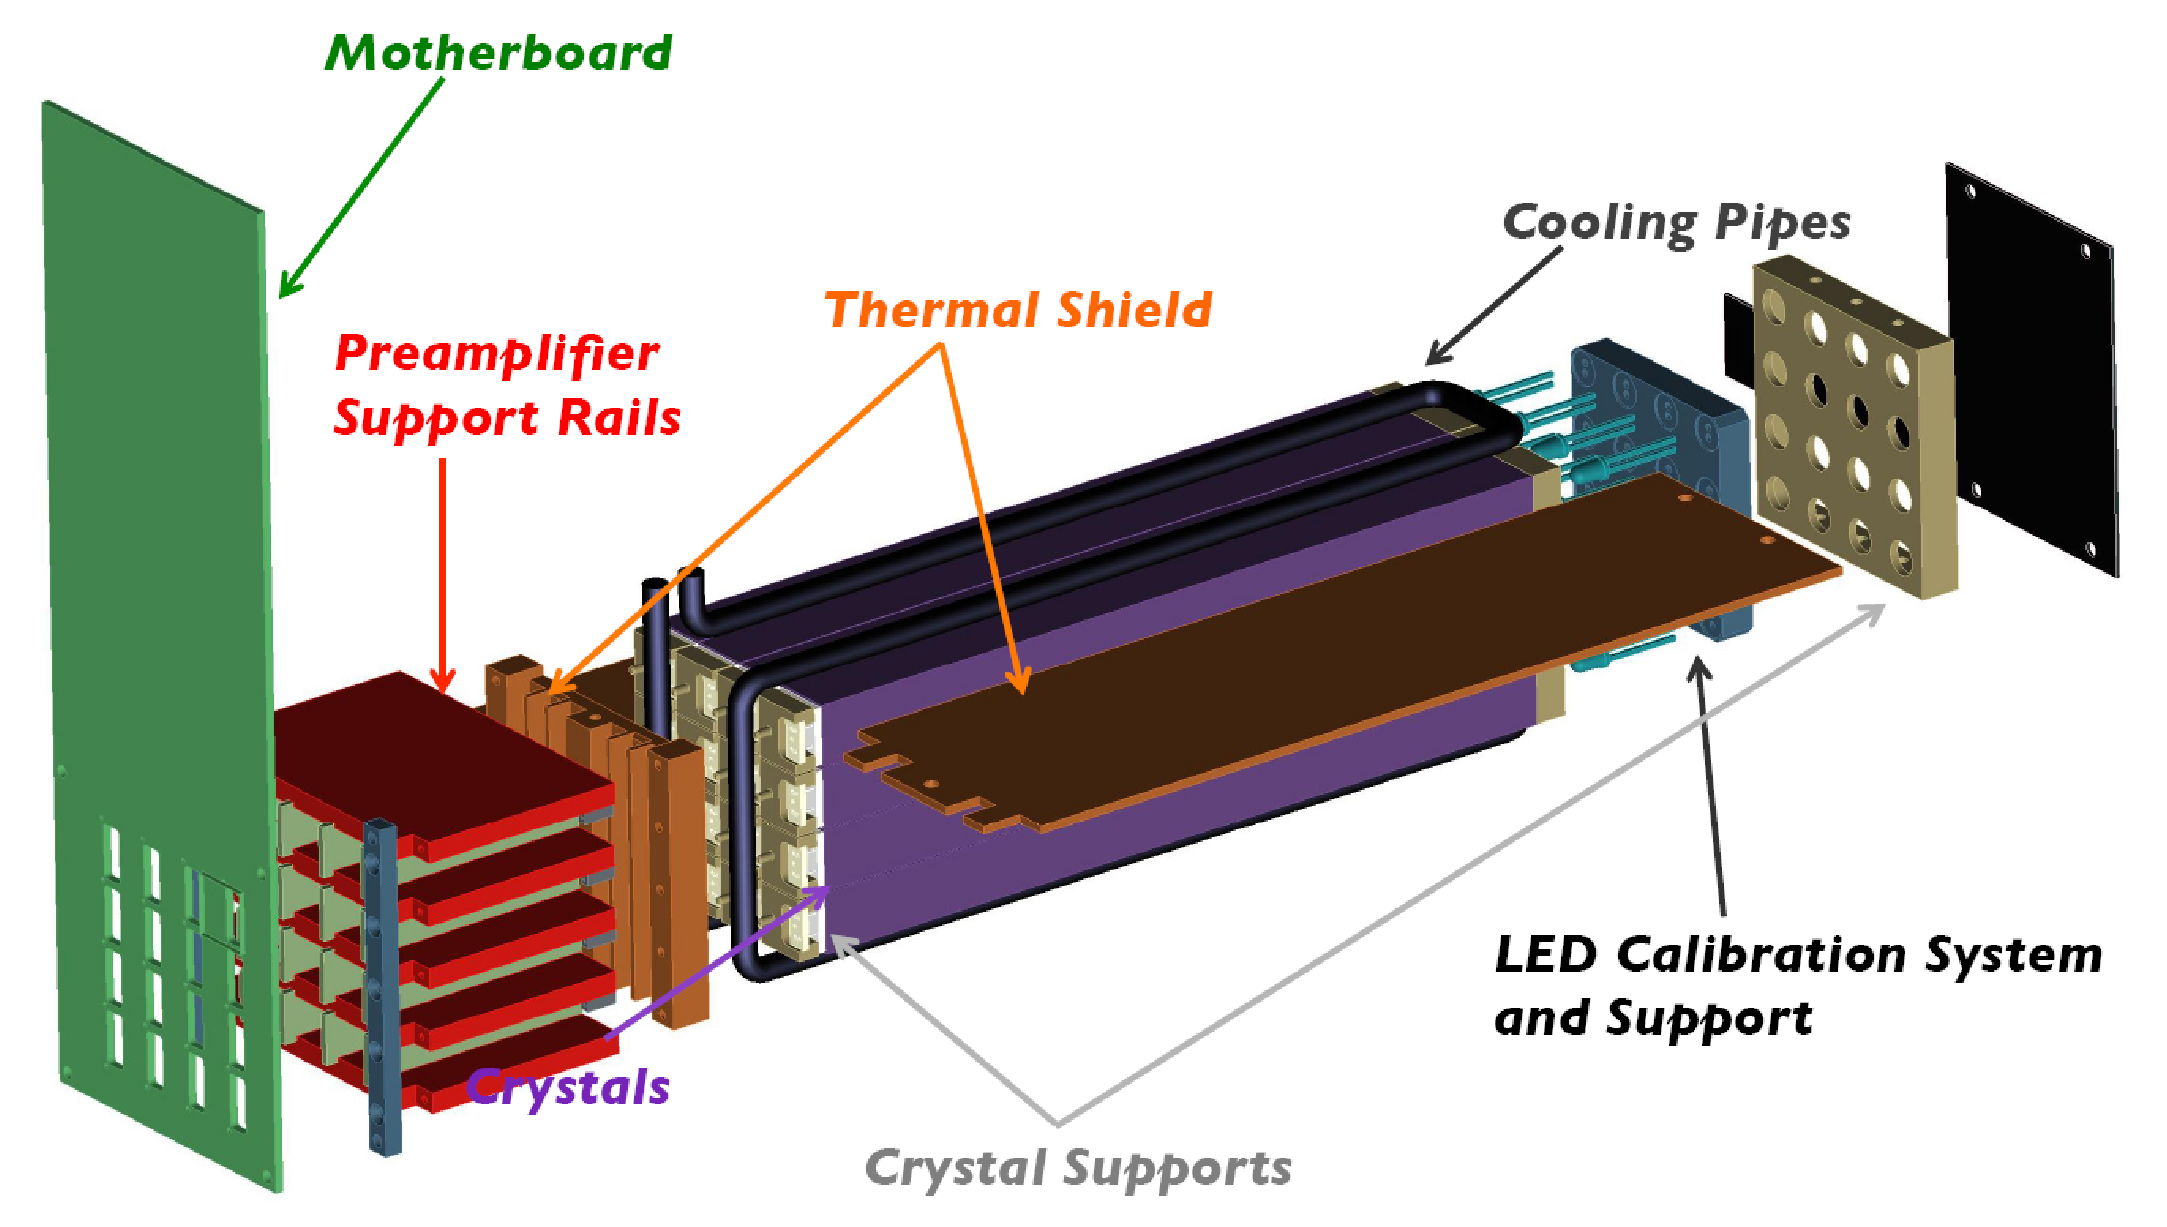
\includegraphics[width=1.0\columnwidth]{./fig/p16-whole.eps}
\caption{Exploded view of the Proto-16 assembly. From left to right, the CAD drawing shows the motherboard, the
  system of copper rails holding the preamplifiers, the copper shield back plate, the crystal assembly, the copper
  shield front plate, and the LED board.}
\label{fig:p16-whole}
\end{figure}

Figure~\ref{fig:btf} shows the BTF experimental hall after the installation of Proto-16 and the associated equipment.
The detector was placed on a movable table that could be displaced in the $x$ and $y$ direction (transverse
plane) with a 0.1-mm accuracy. This feature was exploited to center the calorimeter with respect to the beam. A
plastic scintillator bar, read out by two PMTs, was placed in front of the beam pipe exit window and was used to
determine the arrival time of the electron within the 10-ns bunch duration. The data acquisition system, based on the
JLab CODA standard~\cite{daq}, was triggered by the radio-frequency (RF) signal of the Frascati accelerator. For
each trigger all of the signals of the Proto-16 crystal matrix and of the scintillator-bar PMTs were recorded by
CAEN VME boards. Both the Proto-16 and scintillator signals were sent to a passive splitter whose two outputs were
connected the 250~MHz FADCs and to leading-edge discriminators. The discriminator output was sent to pipeline
TDCs. The samples recorded by the FADCs in an 800~ns window were recorded for each trigger and analyzed offline
to evaluate the charge and time.

\begin{figure}
\includegraphics[width=1.0\columnwidth]{./fig/btf_oct12.eps}
\caption{Experimental setup of the Proto-16 test at the LNF Beam Test Facility (BTF). Beam comes from the right.
  On the left, the detector inside its case (black) is placed on a movable table to allow for centering of the calorimeter
  with respect to the beam. In front of the calorimeter, a plastic scintillator bar wrapped in black Tedlar is used to
  determine the arrival time of the beam electrons.}
\label{fig:btf}
\end{figure}

The conversion between charge and energy was first determined using cosmic ray measurements and then optimized
by studying the response of each crystal to 500~MeV electrons at the LNF-BTF. It is worth noting that the new
calibration constants were found to be within 5-10\% of the initial values determined during cosmic-ray data
taking. The total reconstructed energy  after the full calibration is shown in Fig.~\ref{fig:btf_etot} for an electron
multiplicity of the order of 1-2. The peaks corresponding to different bunch populations are clearly visible and well
separated. 

\begin{figure}
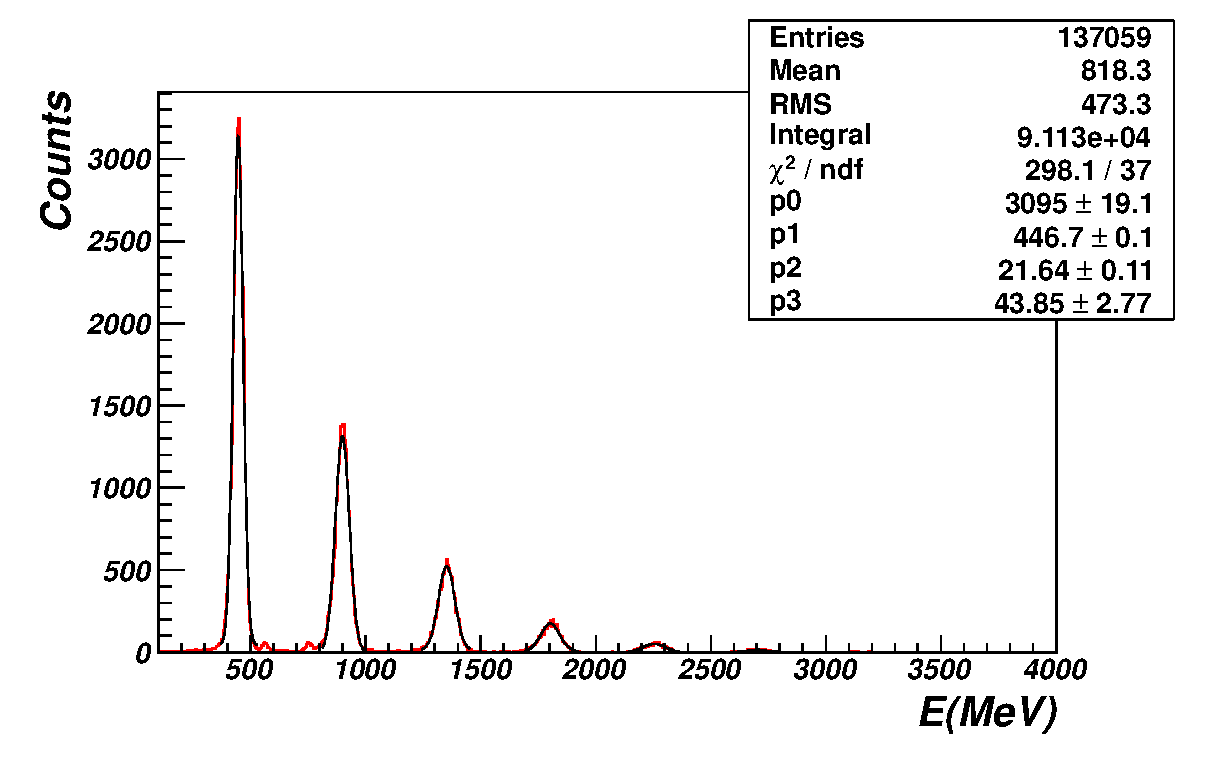
\includegraphics[width=1.0\columnwidth]{./fig/btf_etot_1876_2_6.eps}
\caption{The total energy measured by Proto-16 after calibration. The peaks correspond to different bunch
  populations and are clearly visible and well separated.}
\label{fig:btf_etot}
\end{figure}

\paragraph{Energy Resolution}

The mean values and widths ($\sigma$) of the peaks in the total reconstructed energy spectrum were analyzed to
check the system linearity and to determine the resolution. The measurements were performed by centering the
beam on the calorimeter to have the maximum containment of the electromagnetic shower.
Figure~\ref{fig:btf_linearity} shows the fitted peak position as a function of total energy in the beam bunch for an
APD gain of 150 and a PbWO$_4$ temperature of $18^{\circ}$C. The linear regression of the experimental points
shows no deviations from linearity in the explored range. The same measurement performed in different experimental
configurations gave consistent results, confirming that the system is linear up to the maximum measured energy of
4~GeV.

Figure~\ref{fig:btf_resolution} shows the energy resolution as a function of the energy in the beam bunch. The
colored points correspond to the resolution measured with Proto-16, while the black open circles are the results
of the Monte Carlo (GEMC) simulations. The error bars in the graph show the statistical uncertainty, while the
systematic uncertainty was estimated to be on the order of 5\%.  As expected, the experimental resolution
improves for increasing energy, reaching an asymptotic behavior at about 3~GeV. The measurements performed in
different configurations are in general consistent, varying within a range of 0.5\% except for the resolution obtained
at room temperature and $G$=75 (orange points). The resolution in this case is systematically worse than that
obtained at the same temperature but $G$=150. This was interpreted as due to the preamplifier noise being the
dominant factor in determining the resolution at this temperature. From this we concluded that working at higher
APD gain is the preferable configuration. 

\begin{figure}
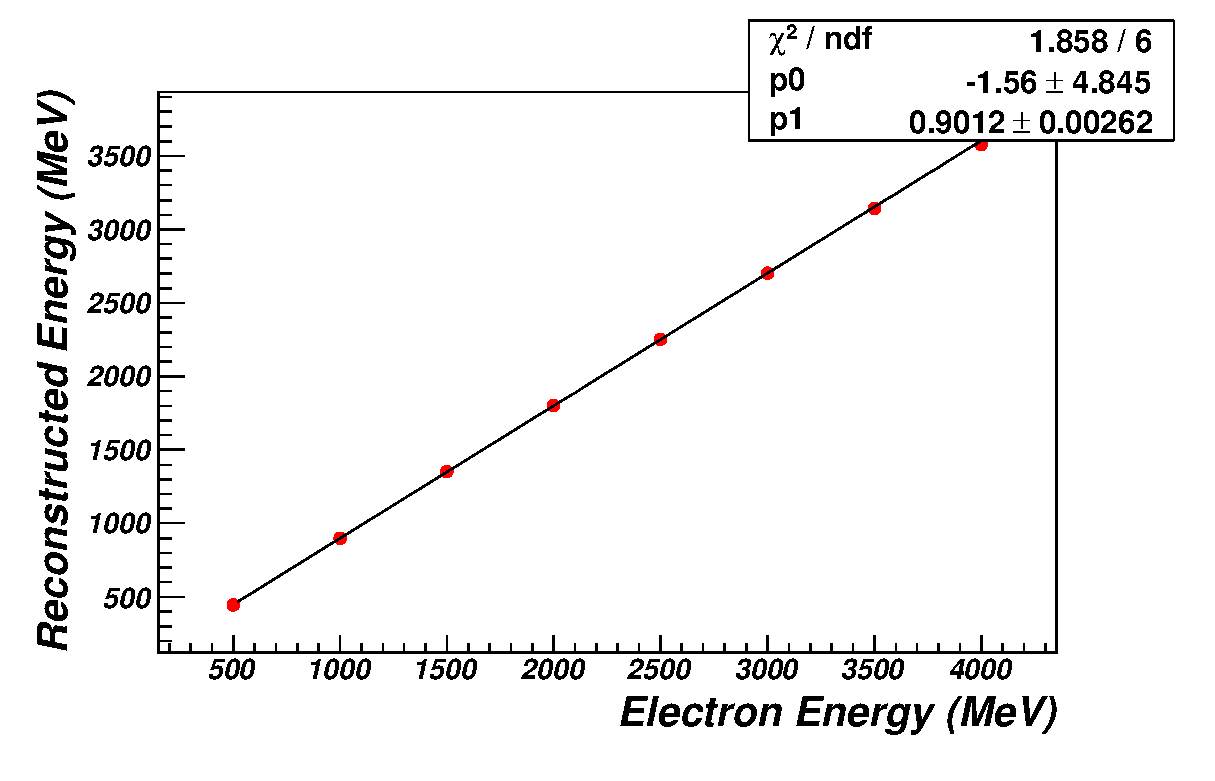
\includegraphics[width=1.0\columnwidth]{fig/btf_linearity_1876_2_6.eps}
\caption{Proto-16 reconstructed energy as a function of the beam bunch energy. The red points were obtained at
  room temperature and with an APD gain of 150. The linear regression of the experimental points shows no deviation
  from linearity.}
\label{fig:btf_linearity}
\end{figure}

The comparison of the resolution obtained at different temperatures shows that lower temperatures,
corresponding to higher light yield, and therefore larger signal, gives better resolution. The best values were
obtained at $-20^{\circ}$C, where the experimental points are in good agreement with the simulation results. The
dependence of the resolution on the temperature is more evident for high bunch energies, where threshold
effects are smaller. Above 2~GeV, the resolution at room temperature seems to be systematically higher than that
obtained at $0^\circ$C or $-20^\circ$C with a difference of about 0.5\%. The difference of the resolution obtained
at $0^\circ$C and $-20^\circ$C is on the contrary negligible within the systematic uncertainties. Based
on these results and considering the technical difficulties in operating the FT-Cal at the lowest temperature, we
concluded that the optimal operating temperature of the calorimeter is $0^\circ$C.

\begin{figure}
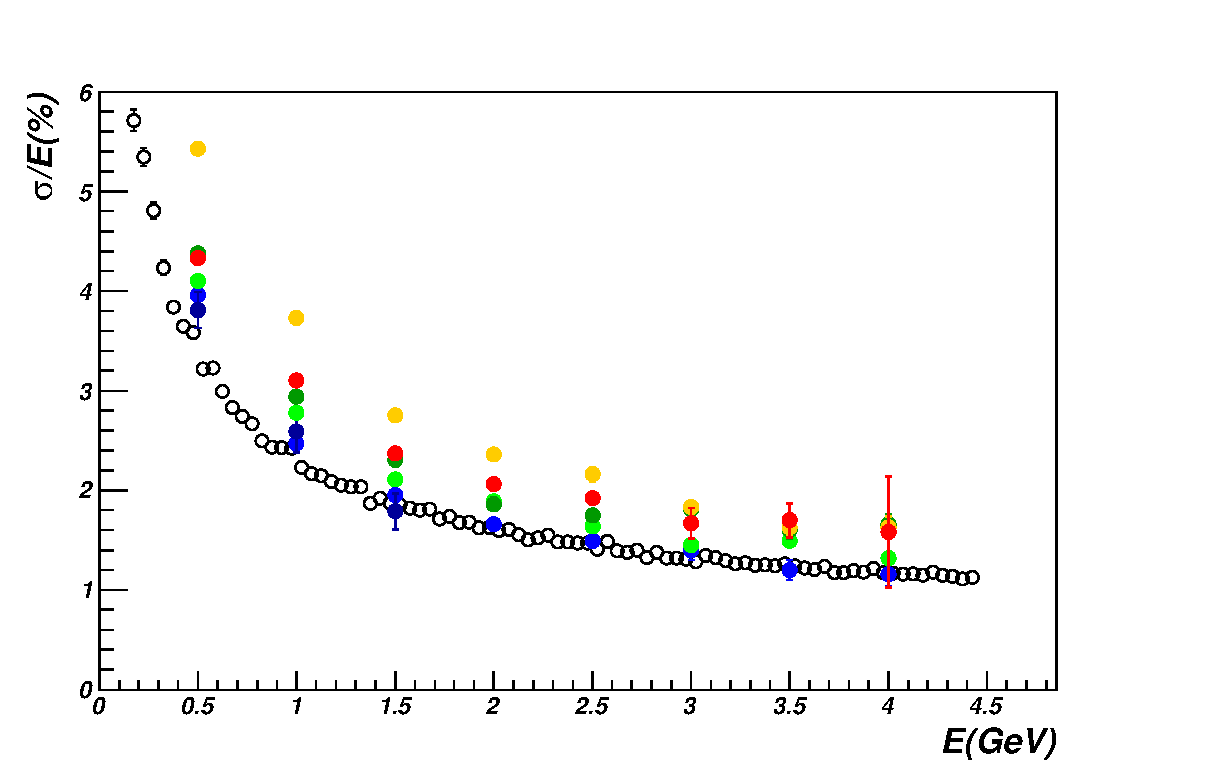
\includegraphics[width=1.0\columnwidth]{./fig/btf_resolution.eps}
\caption{Proto-16 energy resolution as a function of the beam bunch energy. The red and orange points were obtained
  at room temperature for APD gains of 150 and 75, respectively. The green points correspond to $0^\circ$C; the
  darker points were obtained removing the passive splitter. The blue and dark-blue points, that partially overlap, correspond to
  $-20^\circ$C  with APD gains of 150 and 75, respectively. The open black circles show the expected resolution based
  on Monte Carlo simulations. Only statistical uncertainties are shown.}
\label{fig:btf_resolution}
\end{figure} 

\section{Calibration}

torus calibration description


%%%%%%%%%%%%%%%%%%%%%%%%%%%%%%%%%%%%%%%%%%
%% TEX main file for the CLAS12 Nim Papers
%%       Do not edit this file
%%%%%%%%%%%%%%%%%%%%%%%%%%%%%%%%%%%%%%%%%%
\documentclass[review]{elsarticle}
\usepackage{lineno, hyperref, multicol, color, xspace, pdfwidgets, enumerate, amssymb}
\modulolinenumbers[5]
\linenumbers

\journal{Nuclear Instruments and Methods A}

\begin{document}

\begin{frontmatter}
\title{Micromegas Vertex Tracker for CLAS12}

\author[A]{A. Acker} 
\author[A]{D. Atti\'e}
\author[A]{S. Aune}
\author[A]{J. Ball}
\author[A]{P. Baron}
\author[A]{Q. Bertrand}
\author[A]{D. Besin}
\author[A]{T. Bey}
\author[A]{F. Boss\`u}
\author[A]{R. Boudouin}
\author[A]{M. Boyer}
\author[A]{G. Charles}
\author[A]{G. Christiaens}
\author[A]{P. Contrepois}
\author[A]{M. Defurne}
\author[A]{E. Delagnes}
\author[A]{M. Garçon}
\author[A]{F. Georges}
\author[A]{R. Granelli}
\author[A]{N. Grouas}
\author[A]{C. Lahonde}
\author[A]{T. Lerch}
\author[A]{I. Mandjavidze}
\author[A]{O. Meunier}
\author[A]{Y. Mouden}
\author[A]{S. Procureur}
\author[A]{M. Riallot}
\author[A]{F. Sabati\'e}
\author[A]{E. Virique}
\author[A]{M. Vandenbroucke}



\address[A]{Irfu, CEA, Universit\'{e} Paris-Saclay, 91191, Gif-sur-Yvette, France}

\begin{abstract}

For the 12 GeV upgrade of Jefferson Laboratory, a Silicon Vertex Tracker (SVT) has been designed for the CLAS12 spectrometer using single-sided microstrip sensors fabricated by Hamamatsu. The sensors have a graded angle design to minimize dead areas and a readout pitch of 156 $\mu$m, with intermediate strips. Each double-sided SVT module hosts three daisy-chained sensors on each side with a full strip length of 33~cm. There are 512 channels per module, read out by four Fermilab Silicon Strip Readout (FSSR2) chips, featuring data-driven architecture, mounted on a rigid-flex hybrid board. The modules are assembled on the barrel using a unique cantilevered geometry to minimize the amount of material in the tracking volume. This paper is focused on the design, qualification of the performance, and experience in operating and commissioning the tracker during the first year of the data taking.

\end{abstract}

\end{frontmatter}

\date{\today}

\section{Overview}

simulations overview description, how geometry and digitization.

Then we go to each detector

- geometry
- calibration constants
- digitization.





\subsection{Target}

The CLAS12 target components are imported from the engineering model. The STEP files are converted to tessellated STL files and imported
in the GEMC simulation \cite{targetCorrection}, \cite{targetStudy}. An example of the tessellation is shown in \F{targetScatteringChamber}.

Key elements of the STL import include the torlon tube to the target cell,
the target aluminum windows, the Kapton walls, and the scattering chamber, see \F{targetDesign}.
An overview of the target in Geant4 and the engineering model is shown in \F{targetOverview}.

\begin{figure}
	\centering
	\includegraphics[width=0.95\columnwidth,keepaspectratio]{img/targetDesign.png}
	\caption{The CLAS12 target design. Top left: the entry assembly schematic. Top right: the liquid hydrogen cell
            dimensions: the outer radius is tapered down from 15 mm at z=-2.5cm to 10mm at z=2.5mm.
            Bottom left: The cell implementation in GEMC from the CAD drawings. From left to right (beam direction):
            the black torlon tube, the upstream aluminum window, the target cell, the kapton cup and the
				downstream aluminum window. Bottom right: the GEMC implementation of the kapton cup.}
	\label{fig:targetDesign}
\end{figure}


\begin{figure}
	\centering
	\includegraphics[width=0.99\columnwidth,keepaspectratio]{img/targetOverview1.png}
	\includegraphics[width=0.99\columnwidth,keepaspectratio]{img/targetOverview2.png}
	\caption{Top: overview of the target implementation in GEMC includes the scattering chamber (cyan color), the
            downstream cup near the right of the figure and 50 $\mu$m aluminum window. Bottom: the torlon base
            tube starts at a radius of r=6.06 mm, and ends at r = 7.75 mm. It is 63.7 mm long.}
	\label{fig:targetOverview}
\end{figure}

The Github location of the GEMC perl API scripts and the STL files is \url{https://github.com/gemc/detectors/tree/master/clas12/targets}.






\section{Barrel Silicon Vertex Tracker (BST)}

The CLAS12 BST geometry is created using the geometry service (location?)
The geometry directory is "bst".


\subsection{Geometry}

\subsubsection{Geometry Git Location}

\subsection{Process ID}

\subsection{Digitization}


\subsubsection{ADC}
\subsubsection{TDC}

\subsubsection{Summary of CCDB Table used}

\subsection{Digitized Bank}

\subsubsection{Time Window}

\subsubsection{Process Routine Git Repository Location}


The BST hit process routines are located in the repository: \url{https://github.com/gemc/source/tree/master/hitprocess/clas12/svt}

\subsection{Barrel and Forward Micromegas Trackers (BMT and FMT)}

\subsubsection{Geometry}

The Micromegas geometry is implemented through the native GEMC geometry API. There are two subsystems: a ``barrel'' micromegas
between the SVT and the CTOF, made by are three concentric regions divided azimuthally in three identical sectors; and a ``forward'' micromegas
made by three disk regions divided azimuthally in six identical sectors. In both subsystems each region is made by two layers,
one with wires parallel to the beam and one with wires perpendicular to the beam (see \F{bmtGeometry}).
Each micromegas sector contains a cover layer with copper ground, the printed circuit board (PCB) with the readout strips,
the Kapton support, the mesh layer, the ionizing gas, and other layers of material, listed in order below:

\begin{itemize}
	\item overlay
	\item copper ground
	\item PCB
	\item strips
	\item Kapton
	\item gas (amplification gap)
	\item mesh
	\item gas (drift detection gap)
	\item drift potential electrode
	\item foil
	\item ground
\end{itemize}

The sensitive volume contains argon/isobutane gas and is associated with the BMT and FMT hit process routines.
The geometry is summarized in \F{bmtGeometry}. The strip identification is performed in the Process ID routine.

\begin{figure}
	\centering
	\includegraphics[width=0.99\columnwidth,keepaspectratio]{img/bmtGeometry.png}
	\includegraphics[width=0.99\columnwidth,keepaspectratio]{img/bmtDetail.png}
	\caption{Top: a longitudinal cut view of the CLAS12 Central Detector trackers. The target is surrounded by 3 layers of SVT and
            6 layers of micromegas, 3 with $z$-strips, 3 with $c$-strips. On the downstream end (beam incident from the left)
			the Forward Micromegas Tracker disks are visible.
            Bottom: detail of the micromegas GEMC geometry, showing the overlay cover, the copper ground, and the PCB.}
	\label{fig:bmtGeometry}
\end{figure}


\subsubsection{Process ID}
At each Geant4 step, the local coordinates in the sensor volume are used to calculate the strip number.
The algorithm includes the Lorentz angle based on the magnetic field strength, the particle direction,
the pitch angle between the strips, and the dead zones of the sensitive parts.
A virtual electron avalanche is simulated based on the energy deposited. The avalanche
is deposited onto one strip or distributed among several to account for the energy sharing.



\subsubsection{Digitization}

The Micromegas digitization provides the ADC value calculated using the total energy deposited (after hit sharing).
There is no timing information in the output.
The digitized output bank variables are summarized in Table \ref{tab:mmBank}.

\begin{table}[h]
	\begin{center}
		\begin{tabular}{| c | c | c |}
			\hline \hline
			Variable & Description  \\
			\hline
              layer  &      layer number   \\
             sector  &     sector number   \\
              strip  &      strip number   \\
               Edep  &  energy deposited   \\
                ADC  &               ADC   \\
			\hline \hline
		\end{tabular}
	\end{center}
	\caption{The digitized BMT and FMT banks.}\label{tab:mmBank}
\end{table}

The time window  of the Micromegas is set to to 132 ns: all Geant4 steps within the same strip and time window are collected in one hit.


\section{Central Time-Of-Flight (CTOF)}

The CLAS12 CTOF geometry components are imported from the engineering model. The cad files are converted to tessellated STL files.
The geometry directory is "ctof"

\subsection{Geometry}

\subsubsection{Geometry Git Location}

\subsection{Process ID}

\subsection{Digitization}

\subsubsection{Summary of CCDB Table used}

\subsection{Digitized Bank}

\subsubsection{Time Window}

\subsubsection{Process Routine Git Repository Location}



\subsection{Central Neutron Detector}

The Central Neutron Detector (CND)~\cite{cnd-nim} reconstruction service is designed to process raw ADC and TDC information and reconstruct clusters, defined as ensembles of counters matched in space and time. These objects constitute the output of the service that is passed to the Event Builder for particle formation and identification. The algorithm implemented in the service include three steps:

\begin{itemize}
\item{the reconstruction of the time and position of the hit in the paddle;}
\item{the reconstruction of the deposited energy;}
\item{the matching of CND hits with tracks coming from the interaction vertex.}
\end{itemize}

%The reconstruction makes use of the calibration constants of the CND summarized in
%Table~\ref{table_cnd_constants}.
%
%%%%%%%%%%%%%%%%%%%%%%%%%%%%%%%%%%%%%%%%%%%%%%%%%%%%%%%%%%%%
%\begin{table}[htbp]
%\begin{center}
%\begin{tabular}{|c|c|c|} \hline
%Constant Name & Number of Constants  & Units \\ \hline
%$t_{\rm{LR}}$ & 72 & ns\\ \hline
%v_{\rm{eff}}$ & 144 & cm/ns \\ \hline
%$u_{\rm{t}}$ & 72 & ns \\ \hline
%$t_{\rm{LR}_{\rm{ad}}}$ & 72 & ns \\ \hline
%$t_{\rm{off}}$ &72 & ns\\ \hline
%$A_{\rm{L}}$ & 144 & cm\\ \hline
%$MIP_{\rm{D}}$, $MIP_{\rm{I}}$ & 144 each & no units \\ \hline
%\end{tabular}
%\caption{The constants computed in the CND calibration.}
%\label{table_cnd_constants}
%\end{center}
%\end{table}
%%%%%%%%%%%%%%%%%%%%%%%%%%%%%%%%%%%%%%%%%%%%%%%%%%%%%%%%%%%%

%\subsubsection{Timing Calibration}
%
%The paddle in which the hit occurs must be determined before all other reconstruction steps. The raw hit
%times are obtained from the measured TDC channel using a slope constant of 0.0234~ns/channel for all
%channels.
%
%The left and right times of a hit in the left paddle (we label them as $t_{{\rm{L}}/{\rm{L}}}$ and
%$t_{\rm{R}/{\rm{L}}}$ where the first index corresponds to the paddle under exam, while the second indicates
%the paddle in which the primary hit happened) are given by:%
%
%\begin{equation}
%\label{eq_time_hit_lr}
%t_{{\rm{L}}/{\rm{L}}}=t_{\rm{off}}+t_{\rm{tof}}+\frac{z}{v_{\rm{eff}_L}}+t_{\rm{S}}+t_{\rm{off}_{\rm{L}}}+{\rm{TDC}}_{\rm{j}},
%\end{equation}
%
%\begin{equation}
%\label{eq_time_hit_lr1}
%t_{{\rm{R}/{\rm{L}}}}=t_{\rm{off}}+t_{\rm{tof}}-\frac{z}{v_{\rm{eff}_L}}+\frac{L}{v_{\rm{eff}_L}}
%+\frac{L}{v_{\rm{eff}_{\rm{R}}}}+u_{\rm{t}}+t_{\rm{S}}+t_{\rm{off}_{\rm{R}}}+{\rm{TDC}}_{\rm{j}},
%\end{equation}
%
%\noindent
%where $t_{\rm{tof}}$ is the time of flight, $z$ is the position of the hit measured from the upstream end of the
%paddle, $L$ is the length of the paddle, $t_{\rm{S}}$ is the start time of the event, $t_{\rm{off}_{\rm{L}}}$ and
%$t_{\rm{off}_{\rm{R}}}$ are time offsets associated to the left and right coupled paddles, and ${\rm{TDC}}_{\rm{j}}$
%is the TDC clock jitter. Similarly if the hit happened in the right paddle one can write:
%
%\begin{equation}
%  t_{{\rm{L}}/{\rm{R}}}=t_{\rm{off}}+t_{\rm{tof}}-\frac{z}{v_{\rm{eff}_{\rm{R}}}}+\frac{L}{v_{\rm{eff}_L}}
%  +\frac{L}{v_{\rm{eff}_{\rm{R}}}}+u_{\rm{t}}+t_{\rm{S}}+t_{\rm{off}_{\rm{L}}}+{\rm{TDC}}_{\rm{j}},
%\end{equation}
%
%\begin{equation}
%t_{R/R}=t_{\rm{off}}+t_{\rm{tof}}+\frac{z}{v_{\rm{eff}_{\rm{R}}}}+t_{\rm{S}}+t_{\rm{off}_{\rm{R}}}+{\rm{TDC}}_{\rm{j}}.
%\end{equation}
%
%Defining $\Delta$ and $\Delta'$ as:
%
%\begin{equation}
%\Delta=\frac{L}{v_{\rm{eff}_L}}-\frac{L}{v_{\rm{eff}_{\rm{R}}}},
%\end{equation}
%
%\begin{equation}
%\Delta'=t_{\rm{L}/{\rm{X}}}-t_{\rm{R}/{\rm{X}}}+t_{\rm{off}_{\rm{R}}}-t_{\rm{off}_{\rm{L}}},
%\end{equation}
%
%\noindent
%where the index X can be R or L, one can compute $\Delta-\Delta'$ for both cases (hit in the left paddle or hit
%in the right paddle). If the hit is in the left paddle:
%
%\begin{equation}
%\Delta'-\Delta= \frac{2z}{v_{\rm{eff}_L}} - \frac{2L}{v_{\rm{eff}_L}} -u_{\rm{t}} <0.
%\end{equation}

%\noindent
%If the hit is in the right paddle:
%
%\begin{equation}
%\Delta'-\Delta= \frac{2L}{v_{\rm{eff}_{\rm{R}}}}-\frac{2z}{v_{\rm{eff}_{\rm{R}}}} +u_{\rm{t}} >0.
%\end{equation}
%
%\noindent
%If $\Delta'<\Delta$, the paddle in which the hit happened is the left one, otherwise it is the right one.

\subsubsection{Hit Position and Time Reconstruction}

Hit position and time are reconstructed from the TDCs measured for the two PMTs at the ends of the given scintillator paddle. The algorithm is conceptually similar to the one applied to the TOF systems but includes some modification to account for the specific structure and geometry of the detector. The relevant equations are detailed in the following.

{\color{red} REWRITE Starting from $t_{\rm{L}}$ and $t_{\rm{R}}$, defined as the reconstructed hit time from the left and right PMTs,
and subtracting the time offsets obtained from the calibrations, the start time and the time jitter, one can
define the propagation times $t_{\rm{L}_{\rm{prop}}}$ and $t_{\rm{R}_{\rm{prop}}}$ as:

\begin{equation}
t_{\rm{L}_{\rm{prop}}}=t_{\rm{tof}}+\frac{z}{v_{\rm{eff}_{\rm{L}}}},
\end{equation}

\begin{equation}
t_{\rm{R}_{\rm{prop}}}=t_{\rm{tof}}-\frac{z}{v_{\rm{eff}_{\rm{L}}}}+\frac{L}{v_{\rm{eff}_{\rm{L}}}}
+\frac{L}{v_{\rm{eff}_{\rm{R}}}}+u_{\rm{t}}.
\end{equation}

The position of the hit is then obtained as the difference of the propagation times:

\begin{equation}
z=\frac{v_{\rm{eff}_{\rm{L}}}}{2} \left(t_{\rm{L}_{\rm{prop}}}-t_{\rm{R}_{\rm{prop}}}
+ L \cdot \left(\frac{1}{v_{\rm{eff}_{\rm{L}}}}+\frac{1}{v_{\rm{eff}_{\rm{R}}}}\right)  +u_{\rm{t}}\right).
\end{equation}

The $x$ and $y$ coordinates of the hit are obtained from the radius and the azimuthal angle of the hit, which
are, in turn, determined by knowing the layer, sector, and component (left or right) of the hit.  Finally, the time
of flight of the particle that produced the hit is obtained as:

\begin{equation}
t_{\rm{tof}}= \frac{1}{2}\left(t_{\rm{L}_{\rm{prop}}}+t_{\rm{R}_{\rm{prop}}}- L \cdot \left(\frac{1}{v_{\rm{eff}_{\rm{L}}}}
+\frac{1}{v_{\rm{eff}_{\rm{R}}}}\right)  -u_{\rm{t}}\right).
\end{equation}}

\subsubsection{Energy Reconstruction}
{\color{red} REWRITE 
For hits in the left paddle, the two associated ADCs can be written as:

\begin{equation}
\label{eq_rec_3}
ADC_{\rm{L}}=\frac{E_{\rm{L}}}{E_0}\cdot MIP_{\rm{D}}\cdot e^{\frac{-z}{A_{\rm{L}}}},
\end{equation}

\begin{equation}
\label{eq_rec_4}
ADC_{\rm{R}}=\frac{E_{\rm{R}}}{E_0}\cdot MIP_{\rm{I}}\cdot e^{\frac{-(L-z)}{A_{\rm{L}}}},
\end{equation}

\noindent
where $E_{L/R}$ is half the energy deposited by the particle in the left/right paddle and $E_0$ is given by
Eq.~\ref{eq_def_e0}.

\begin{equation}\label{eq_def_e0}
E_0=\frac{h\cdot 1.956}{2}~\rm{MeV},
\end{equation}

\noindent
where $h$ is the thickness of each scintillator. The above equations are valid for hits in the left paddles, while
for hits in the right paddles, the applicable equations are obtained by switching the $L/R$ indices. From
Eqs.~\ref{eq_rec_3} and \ref{eq_rec_4} follows the relations:

\begin{equation}
E_{\rm{L}}=\frac{ADC_{\rm{L}} \cdot E_0}{MIP_{\rm{D}}}\cdot e^{\frac{z}{A_{\rm{L}}}},
\end{equation}

\begin{equation}
E_{\rm{R}}=\frac{ADC_{\rm{R}} \cdot E_0}{MIP_{\rm{I}}}\cdot e^{\frac{L-z}{A_{\rm{R}}}}.
\end{equation}

\noindent
The total deposited energy is given by the sum of $E_{\rm{L}}$ and $E_{\rm{R}}$:

\begin{equation}
E_{\rm{dep}}=E_{\rm{L}}+E_{\rm{R}}.
\end{equation}

}

\subsubsection{Clustering algorithm}
%\subsubsection{Hit/Track Matching}
%Tracks from charged particles crossing the CLAS12 Central Vertex Tracker (CVT) are associated to hits in the CND. This allows, for each CND hit matched with a CVT track, to calculate the position of the hit from the extrapolated track, the pathlength between the track vertex and the hit and the path travelled in the hit paddle. This information is used in the calibration, as well as to veto charged particles when looking for neutrons in the CND. CVT tracks are extrapolated to radii corresponding to the entry point, middle point and exit point of the track in the paddle. These points are defined as the intersections between the helix of the track and cylinders of radii corresponding to the distances between the center of the CD and the three CND layers. A CVT track and a CND hit are matched if the hit coordinates ($x$, $y$, and $z$) and the extrapolated coordinates ($x_m$, $y_m$, and $z_m$) verify the relations:

%\begin{equation}
%\mid x-x_m \mid < \sigma_x ,~~~~\mid y-y_m \mid < \sigma_y , ~~~~z_m % \in [-\sigma_z,L+\sigma_z],
%\end{equation}

%\noindent
%where $\sigma_z=1.5$~cm, $ L$ is the length of a paddle, and $\sigma_x$ and $\sigma_y$ are given by:

%\begin{equation}
%\sigma_x= \sqrt{x^2\frac{\sigma_R^2}{R^2}+y^2\sigma_\phi^2},~~~~
%\sigma_y= \sqrt{y^2\frac{\sigma_R^2}{R^2}+x^2\sigma_\phi^2},
%\end{equation}

%\noindent
%where $R$ is the radius of the hit, $\sigma_R$ is half the thickness of a paddle (1.5~cm) and $\sigma_\phi$ is the azimuthal resolution of each paddle (3.75$^\circ$). The path travelled by the particle in the paddle is approximated as the distance between the entry and exit points. The path length between the vertex and the hit is given by the helix parameters.

\section{High Threshold Cerenkov Counter (HTCC)}

The CLAS12 HTCC geometry is created using the native gemc geometry API.
The geometry directory is "micromegas"


\subsection{Geometry}

\subsubsection{Geometry Git Location}
The github location of the gemc perl api script is \url{https://github.com/gemc/detectors/tree/master/clas12/htcc}.

\subsection{Process ID}
\subsubsection{ADC}
\subsubsection{TDC}

\subsection{Digitization}


\subsubsection{Summary of CCDB Table used}

\subsection{Digitized Bank}

\subsubsection{Time Window}

\subsubsection{Process Routine Git Repository Location}


The HTCC hit process routine location in git is \url{https://github.com/gemc/source/blob/master/hitprocess/clas12/htcc_hitprocess.cc}

\section{Forward Tagger (FT)}


\subsection{Geometry}

\subsubsection{Geometry Git Location}
The github location of the gemc perl api script is \url{https://github.com/gemc/detectors/tree/master/clas12/ft}.

\subsection{Process ID}

\subsection{Digitization}


\subsubsection{ADC}
\subsubsection{TDC}

\subsubsection{Summary of CCDB Table used}
\paragraph(Calorimeter)
\begin{itemize}
	\item /calibration/ft/ftcal/status
	\item /calibration/ft/ftcal/noise
	\item /calibration/ft/ftcal/charge\_to\_energy
	\item /calibration/ft/ftcal/time\_offsets
	\item /daq/tt/ftcal
\end{itemize}
\paragraph(Hodoscope)
\begin{itemize}
	\item /calibration/ft/fthodo/status
	\item /calibration/ft/fthodo/noise
	\item /calibration/ft/fthodo/charge\_to\_energy
	\item /calibration/ft/fthodo/time\_offsets
	\item /daq/tt/fthodo
\end{itemize}



\subsection{Digitized Bank}

\subsubsection{Time Window}

\subsubsection{Background merging algorithm}

\subsubsection{Process Routine Git Repository Location}
The FT hit process routines are: \url{https://github.com/gemc/source/blob/master/hitprocess/clas12/ft_cal_hitprocess.cc} and
\url{https://github.com/gemc/source/blob/master/hitprocess/clas12/ft_hodo_hitprocess.cc}.

\section{Drift Chambers (DC)}

\subsection{Geometry}

The FTOF geometry is implemented through the COATJAVA geometry service.
The service provides the geant4 definitions that are read by the GEMC perl api to build the geometry database.

Each layer is a generic G4Trapezoid, tilted by $+6^O$ or $-6^O$ depending if they are part of a stereo superlayer or not.
The 12 layers in each region (6 per superlayer) are placed in a region mother volume made of air, see \F{dcGeometry}.

\begin{figure}
	\centering
	\includegraphics[width=0.95\columnwidth,keepaspectratio]{img/dcGeometry.png}
	\includegraphics[width=0.95\columnwidth,keepaspectratio]{img/dcDetail.png}
	\caption{Top: the GEMC implementation of the FTOF geometry. The paddles are G4Boxes, embedded in trapezoid representing the mother volumes of each panel.
            Bottom: a zoom-in of the implementation shows the details of the individual paddles for Panel 1B (green) and Panel 1A (purple) }
	\label{fig:dcGeometry}
\end{figure}


\subsubsection{Geometry Git Location}

\subsection{Process ID}

\subsection{Digitization}



\subsubsection{ADC}
\subsubsection{TDC}

\subsubsection{Summary of CCDB Table used}

\subsection{Digitized Bank}

\subsubsection{Time Window}

\subsubsection{Process Routine Git Repository Location}


The DC hit process routine location in git is \url{https://github.com/gemc/source/blob/master/hitprocess/clas12/dc_hitprocess.cc}

\section{Low Threshold Cherenkov Counter}


\subsection{Geometry}

\subsubsection{Geometry Git Location}
The github location of the gemc perl api script is \url{https://github.com/gemc/detectors/tree/master/clas12/ltcc}.

\subsection{Process ID}

\subsection{Digitization}


\subsubsection{ADC}
\subsubsection{TDC}

\subsubsection{Summary of CCDB Table used}

\subsection{Digitized Bank}

\subsubsection{Time Window}

\subsubsection{Process Routine Git Repository Location}


The LTCC hit process routine location in git is \url{https://github.com/gemc/source/blob/master/hitprocess/clas12/ltcc_hitprocess.cc}

\section{}


\subsection{Geometry}

The FTOF geometry is implemented through the COATJAVA geometry service.
The service provides the geant4 definitions that are read by the GEMC perl api to build the geometry database.

All scintillators are geant4 volumes.
Each scintillator is a G4Box embedded in a G4Trapezoid mother volume made of air, see \F{ftofGeometry}.

\begin{figure}
	\centering
	\includegraphics[width=0.95\columnwidth,keepaspectratio]{img/ftofGeometry.png}
\caption{Cherenkov light yield as a function of pion momentum and photon wavelength. The study took into account: the mirror reflectivity; the number of reflections on the mirror and Winston Cones;
the gas refraction index and the gas reflectivity as a function of wavelength; the PMT quantum efficiency; different improvements to optics and PMTs response increase. }
	\label{fig:ftofGeometry}
\end{figure}


\subsubsection{Geometry Git Location}
The github location of the gemc perl api script is 

\subsection{Calibration Constants}

\subsubsection{Summary of CCDB Table used}

\subsection{Digitization}

\subsection{Process ID}

\subsubsection{Time Window}

\subsubsection{Process Routine Git Repository Location}



\subsection{Electromagnetic Calorimeter (EC) and Pre-Shower Calorimeter (PCAL)}

\subsubsection{Geometry}

Both the EC and PCAL (referred to together as ECAL) calorimeter geometry is implemented through the java geometry service.
The service provides the Geant4 definitions that are read by the GEMC perl API to build the geometry database.

All scintillators are Geant4 volumes. The paddles are assigned the scintillator material and associated with the ECAL hit process routine.
Each scintillator is a trapezoid embedded in a trapezoid mother volume made of air (\F{ecGeometry}).

\begin{figure}
	\centering
	\includegraphics[width=0.99\columnwidth,keepaspectratio]{img/ecGeometry.png}
	\includegraphics[width=0.99\columnwidth,keepaspectratio]{img/ecDetail.png}
	\caption{Top: a 4 GeV electron track (dotted line) showering in the GEMC implementation of the ECAL geometry.
        	 Beam is incident from the left.
             The scintillator layers alternate with a layer of lead, for a sampling fraction of about 0.3.
             Bottom: a zoom-in transverse view of the electron shower.}
	\label{fig:ecGeometry}
\end{figure}

%\begin{figure}
%	\centering
%	\includegraphics[width=0.99\columnwidth,keepaspectratio]{img/pcalGeometry.png}
%	\includegraphics[width=0.99\columnwidth,keepaspectratio]{img/pcalDetail.png}
%	\caption{Top: a 4 GeV $\pi^0$ decayed in two photons hitting the GEMC implementation of the PCAL geometry.
%           The paddles are G4Boxes, embedded in trapezoid representing the mother volumes of each panel.
%            The paddles layers are alternating with trapezoid made of lead, for a sampling fraction of about 0.3.
%            Bottom: a zoom-in transverse view of showers.}
%	\label{fig:pcalGeometry}
%\end{figure}

\subsubsection{Digitization}
The digitization is the same for both the EC and the PCAL calorimeters.
The energy deposited is reduced based on the position on the scintillator using the calibrated attenuation length.
A number of photoelectrons is generated using a Poissonian distribution based on the attenuated energy.
The scintillator resolution $\sigma_{res}$ is obtained from the calibration constants, after the fluctuations in PMT gain
are taken into account using a Gaussian form with $\sigma_{res}$. A conversion factor is used to produce an ADC output.

The absolute hit time is corrected using the attenuation length and an additional factor that accounts for the time-walk correction.
The digitized output bank variables for both systems are summarized in Table \ref{tab:ecBank}.

\begin{table}[h]
	\begin{center}
		\begin{tabular}{| c | c | c |}
			\hline \hline
			Variable &                Description   \\
			\hline
             sector  &              sector number   \\
              stack  &  scintillator layer number   \\
               view  &                       view   \\
              strip  &               strip number   \\
                ADC  &                        ADC   \\
                TDC  &                        TDC   \\
               hitn  &                 hit number   \\
			\hline \hline
		\end{tabular}
	\end{center}
	\caption{The digitized EC and PCAL banks.}\label{tab:ecBank}
\end{table}


The time window of both PCAL and EC is set to 400~ns: all Geant4 steps within the same paddle and time window are collected in one hit.

\section{Solenoid and Torus Magnets}


\subsection{Geometry}
The solenoid geometry is produced with the GEMC perl api. The solenoid is a single polycone volume, shown in \F{solenoid}
in a section view with the target and an 11 GeV electron beam.

\begin{figure}
	\centering
	\includegraphics[width=0.98\columnwidth,keepaspectratio]{img/solenoid.png}
   \caption{An 11 GeV electron beam is impinging on a 5 cm liquid hydrogen target. At the full $10^{35} cm-2s-1$ luminosity, this correspond to
            124,000 electrons in a 250 ns window. Normally this would produce a storm of Moeller electrons that would saturate any detector in the forward or central
				region. However the solenoid focus all of the Moeller electrons along the beam line, providing a most effective shield for CLAS12.
            }
	\label{fig:solenoid}
\end{figure}

The torus geometry is imported from the engineering CAD model through 54 tessellated volumes. Among the volumes:

\begin{itemize}
	\item the bore heat shield and hub components
	\item the back and front hub steel plates
	\item the stainless steel coil vacuum jackets
	\item the torus coils containing the wires, represented by copper volumes in geant4
\item internal shielding around the hub, made by tungsten cylinders (blue in \F{torus})
\end{itemize}

The torus hub is protected from the beampipe background with additional tungsten shielding.
The torus geometry is shown in \F{torus}.

\begin{figure}
	\centering
	\includegraphics[width=0.95\columnwidth,keepaspectratio]{img/torusGeometry.png}
	\includegraphics[width=0.95\columnwidth,keepaspectratio]{img/torusDetail.png}
	\caption{Top: the GEMC implementation of the torus hardware. The volumes are imported from the CAD engineering model.
            The stainless steel vacuum jacket embeds the geant4 coil volumes.
				Bottom: a section view of the torus in the vicinity of the beamline. The warm and cold hub are visible, along with the
				tungsten shielding (blue colors).}
	\label{fig:torus}
\end{figure}


\subsection{Magnetic Field Maps} \label{clas12FieldMaps}


The field maps are imported into the simulation using ascii files. Both fields can be scaled by an arbitrary number.
Both fields are defined in the Hall B coordinate system and both can be shifted and tilted by additional delta amounts.

\subsubsection{Solenoid}
The solenoid field map has cylindrical symmetry around the z- axis, so the map used in the simulation is defined in the transverse / longitudinal plane
and then rotated when requested by the Geant4 navigation. The integration method used in the simulation is the Runge-Kutta 4.

The solenoid field near the target is parallel to the z-axis and its uniformity was measured to be 318 ppm over a 25mm diameter and 40mm long cylindrical volume.
The field map grid is made by 600 points in the transverse coordinate, from 0 to 3m and by 1200 points
along the z-axis, from \mbox{-3m} to 3m.
The field grid values are linearly interpolated to the (x,y,z) coordinate requested by geant4.

Table \ref{tab:solMap} shows the field map ascii data structure.


\begin{table}[h]
	\begin{center}
		\begin{tabular}{| c | c | c | c |}
			T (m)  & Z (m) &  $B_T $  & $ B_L $ \\
			\hline
          0.005  &  -0.025 & 0.000013  & 5.000880 \\
          0.005  &  -0.020 & 0.000044  & 5.000822 \\
          0.005  &  -0.015 & 0.000073  & 5.000704 \\
          0.005  &  -0.010 & 0.000101  & 5.000529 \\
          0.010  &  -0.025 & 0.000028  & 5.000928 \\
          0.010  &  -0.020 & 0.000089  & 5.000867 \\
          0.010  &  -0.015 & 0.000148  & 5.000747 \\
          0.010  &  -0.010 & 0.000203  & 5.000570 \\
		\end{tabular}
	\end{center}
\caption{Solenoid ascii field map values around the target. T is the transverse coordinate $\sqrt{(x^2+y^2)}$ and z is the longitudinal coordinate.
            The solenoid field is centered at Z=0, the location of the center of the target. The field values are in Tesla.}\label{tab:solMap}
\end{table}

\subsubsection{Torus}
The torus field can be imported using a symmetric map or a full 3D map.
The symmetric map is defined in half the CLAS12 sector. It is symmetric around the sector mid-plane and copied in each sector
when requested by the Geant4 navigation. The 3D map covers the entire cartesian space and accounts for field deviations due to coil
movements or imperfections \cite{GhoshalSolenoid}.


The field map has 251 points along the z-axis, from 1m to 3m. It has 2501 points in the transverse coordinate, from 0 to 5m.
It has 16 azimuthal points from $0$ to $30^0$. The field grid values are linearly interpolated to the (x,y,z) coordinate requested by geant4.

The torus field in mid sector is perpendicular to the z-axis and is typically $2.058$ Tesla.
Table \ref{tab:torMap} shows the field map ascii data structure.

\begin{table}[h]
	\begin{center}
		\begin{tabular}{| c | c | c | c | c | c | }
         $\phi$ (deg) & T (m)    & Z (m)    &  $B_x $  &    $B_y$    & $B_z$\\
			\hline
          0.0         &  190.0   &  338.0   &  0       &     0.451275 &  0 \\
          0.0         &  190.0   &  340.0   &  0       &     0.450136 &  0 \\
          0.0         &  190.0   &  342.0   &  0       &     0.448789 &  0 \\
          0.0         &  190.0   &  344.0   &  0       &     0.447235 &  0 \\
          0.0         &  190.0   &  346.0   &  0       &     0.445472 &  0 \\
          0.0         &  190.0   &  348.0   &  0       &     0.443502 &  0 \\
          0.0         &  190.0   &  350.0   &  0       &     0.441323 &  0 \\
          0.0         &  190.0   &  352.0   &  0       &     0.438935 &  0 \\
		\end{tabular}
	\end{center}
	\caption{Torus ascii field map values near mid-sector. T is the transverse coordinate $\sqrt{(x^2+y^2)}$ and z is the longitudinal coordinate.
            The field values are in Tesla.}\label{tab:torMap}
\end{table}


\subsubsection{Geometry Location on GitHub}
The Github location of the GEMC perl API script for the solenoid and the torus CAD volumes is \url{https://github.com/gemc/detectors/tree/master/clas12/magnets}.


\section{Beamline and Shielding}

\subsection{Geometry}

\subsubsection{Geometry Git Location}


\section{Summary of geometry and digitization}


\section{Signals and Readout}

solenoid Signals and Readout description


\section{Performance}

ec performance description


\section{Distribution and Documentation}

The GEMC framework is documented on the GEMC website \cite{GEMC}. This includes the latest news and releases,
examples, procedure details, and documentation for all the available options.
The software is distributed in two ways: with docker, or by downloading the source from the public git repository.


A docker container with the necessary libraries to run GEMC and the reconstruction software
is created in the JeffersonLab hub repository \cite{jlabDocker}.
The container is tagged, and every tag contains a set version of these libraries:

\begin{itemize}
	\item pythia-based event generators for various physics channels relevant to the CLAS12 analyses;
	\item GEMC with the CLAS12 geometry;
	\item the java reconstruction software \cite{recon-nim}.
\end{itemize}


The code git repository is \url{https://github.com/gemc/source}, which is a public repository.
The development contribution mechanism is illustrated in \F{github}: collaborators fork the repository
and make pull requests that are validated by the code author.
GEMC is released on a semi-annual cycle.

\begin{figure}
	\centering
	\includegraphics[width=0.99\columnwidth,keepaspectratio]{img/github.png}
	\caption{Typical workflow of contribution to the code. First, the main repository is forked and worked on. Then, during the fork code developments,
	         comments can be made on the various commits. Lastly, when the users make the pull request, the changes are validated and then merged
             to the master repository (or sent back with comments if there were problems).}
	\label{fig:github}
\end{figure}


The list of software packages included in the GEMC framework is:

\begin{itemize}
	\item clhep: Class Library for High Energy Physics \cite{clhep};
	\item xercesc: validating XML parser \cite{xercesc};
	\item Geant4: the libraries to simulate the passage of particles through matter \cite{geant4};
	\item qt: a C++ graphic library \cite{qt};
	\item evio: the CLAS12 data format \cite{evio};
	\item CCDB: the calibration database based on mysql \cite{ccdb}.
\end{itemize}

The main documentation is on the GEMC website \cite{GEMC}. It includes examples of how to create and run a custom geometry
and use various features like event generators, geometry factories, hit definitions, output, etc.

The CLAS12 development of both hit process routines and geometry is kept on the CLAS12 tags portal \cite{clas12Tags},
which also contains documentation on how to run with configurations corresponding to the various experiments, how to change the
beamline configuration, and how to switch between code and geometry releases.






\section{Conclusions}

To address the change of its scope from electron to pion identification for momenta greater than 3.5~GeV,
the original CLAS Cherenkov Counters were refurbished at part of the new CLAS12 Low Threshold Cherenkov
Counter (LTCC) system. The work included improvements of the reflectivities for the mirrors and the Winston
cones, p-terphenyl coating of the PMTs, expansion of the gas volumes, and redesign of the box walls and patch
panels. The LTCC detector sectors after refurbishment are shown in \F{ltccInstalled} installed on the CLAS12
Forward Carriage upstream of the Forward Time-of-Flight system. The average LTCC efficiency for electron
detection in the momentum range from 3.5 to 6.5~GeV is 94\%. The pion efficiency starts around 50\% near
the expected signal threshold, and rises with momentum as expected. A plateau of 88\% is reached at a momentum
of 5~GeV. This is within range of an expectation of efficiency above 90\%. Additional future studies are required
to full quantify the detection efficiency of the CLAS12 LTCC for both positive and negative pions as a function of
momentum.

\begin{figure}
    \centering
    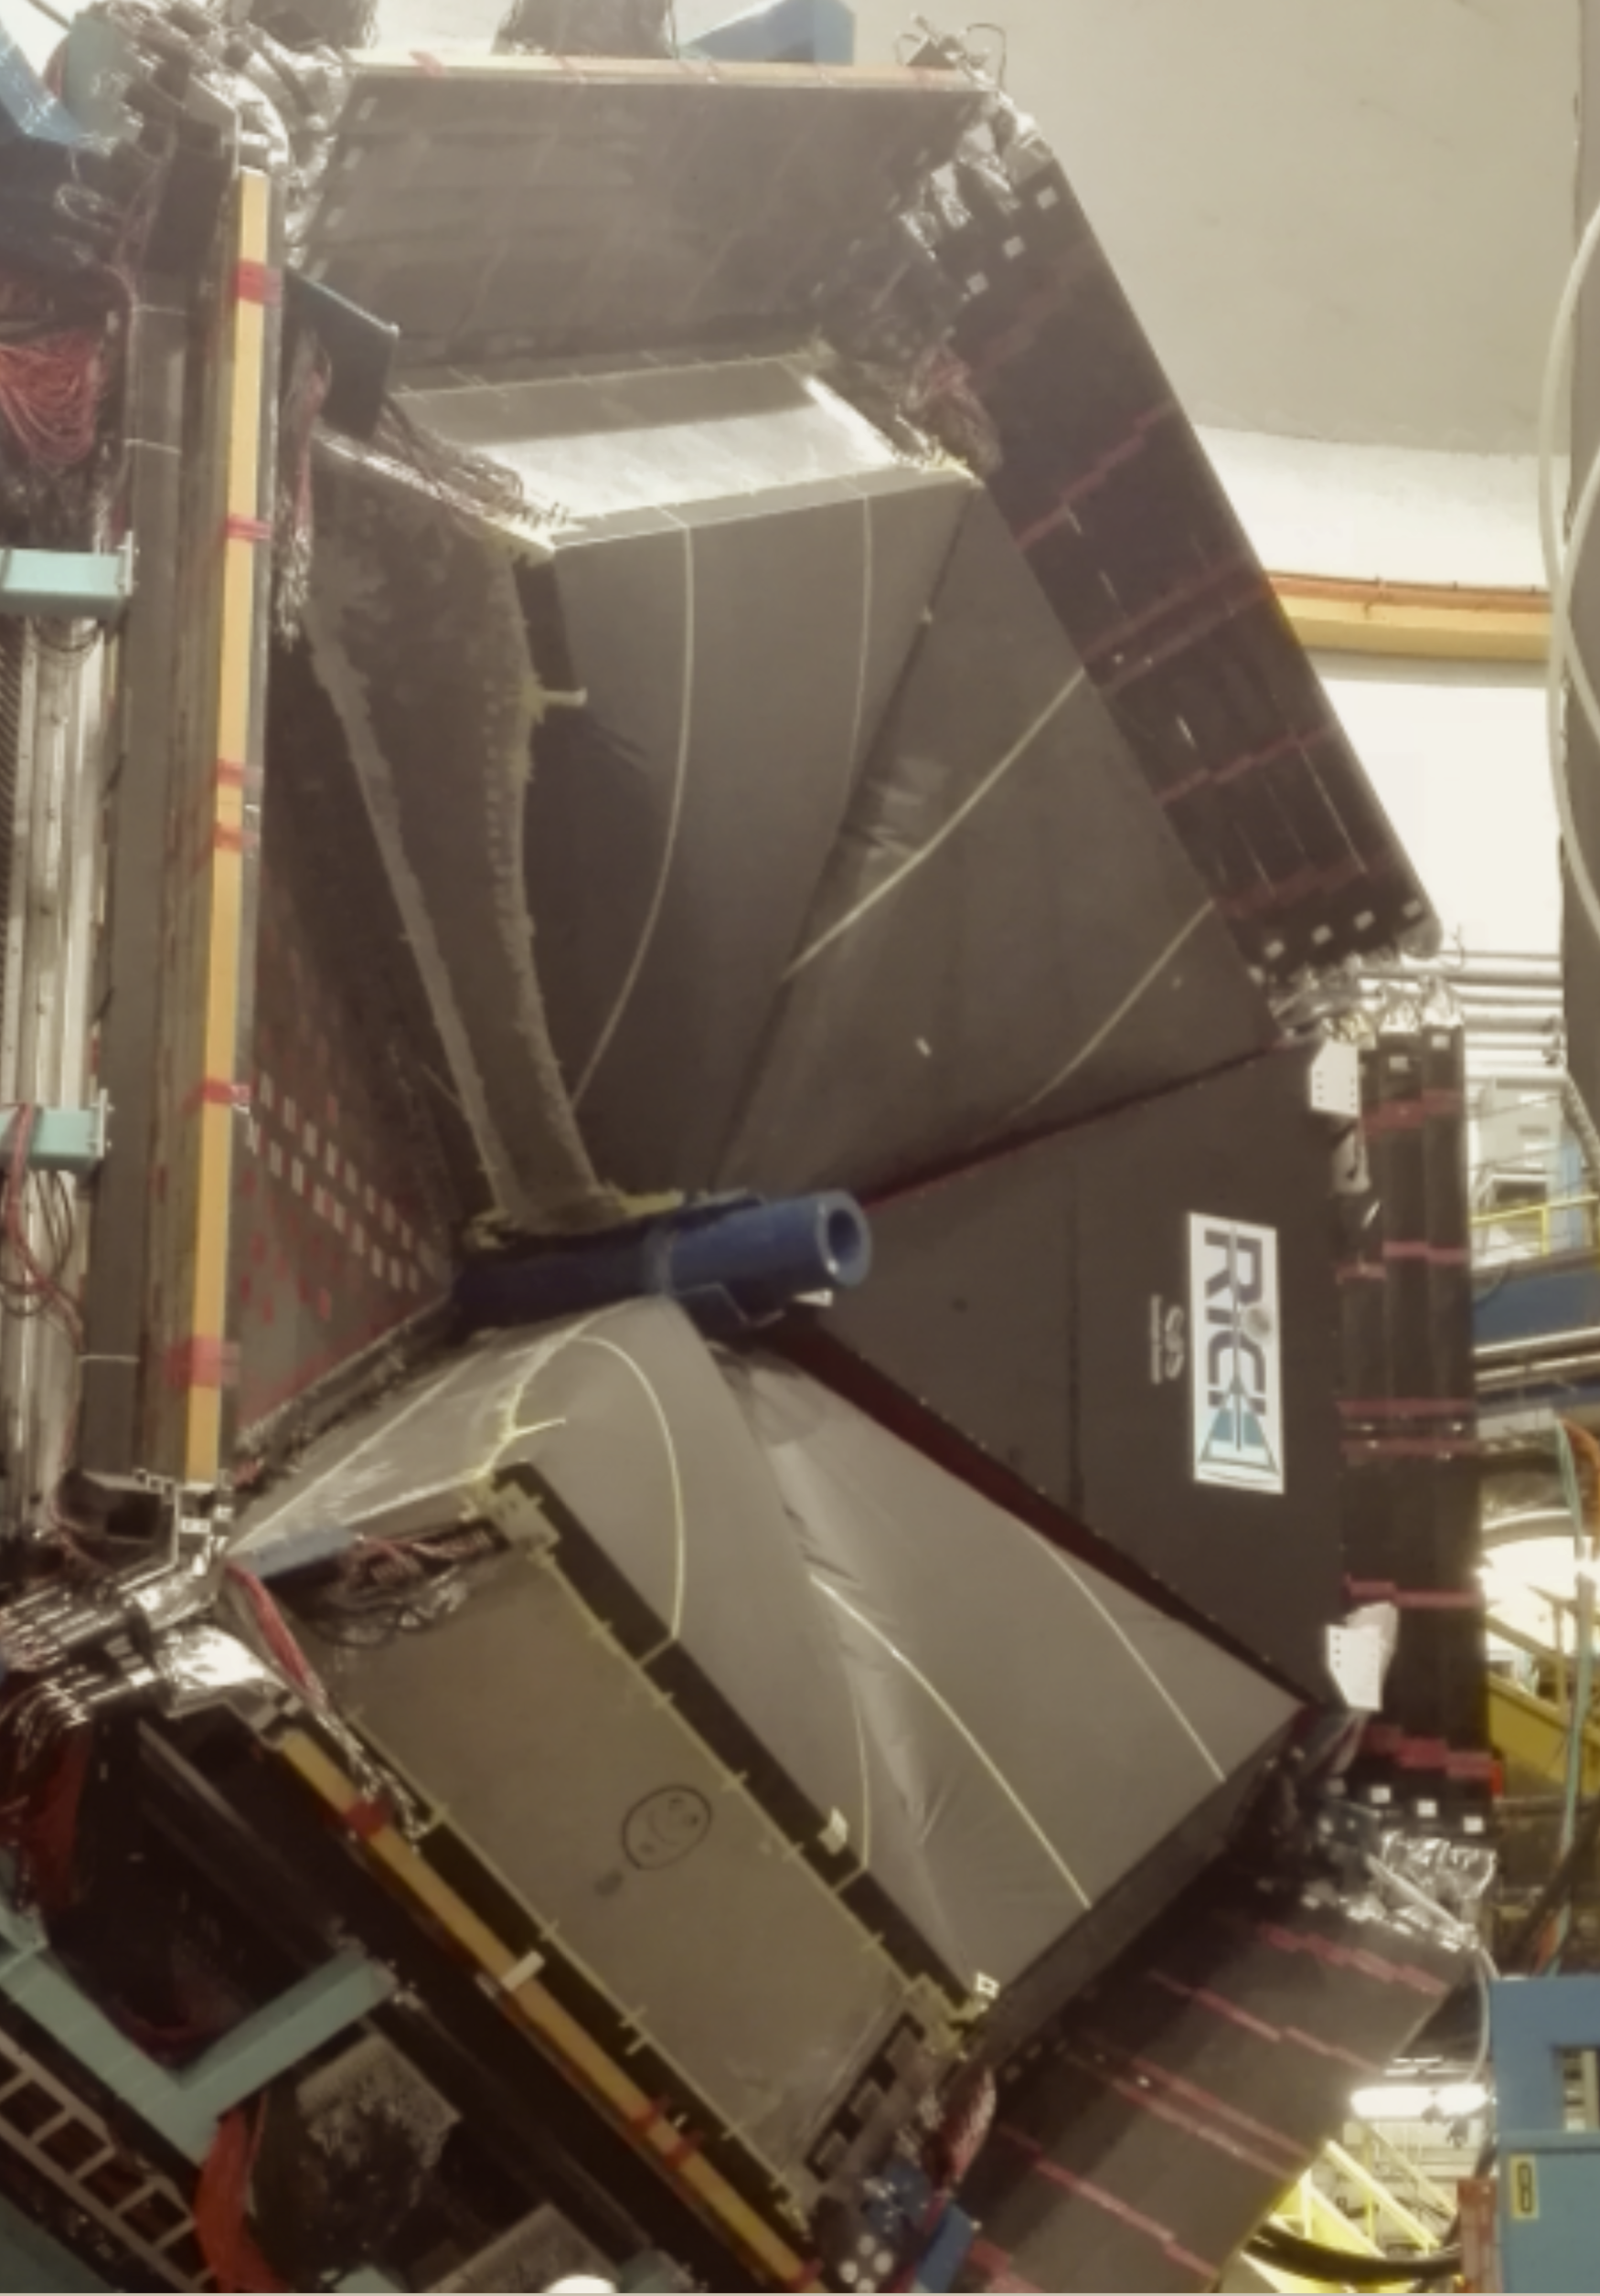
\includegraphics[width=1.0\columnwidth,keepaspectratio]{img/ltccInstalled.png}
    \caption{The LTCC sectors installed after refurbishment on the CLAS12 Forward Carriage. The RICH detector
    is installed in the sector~4 position and the sector~1 position awaits the installation of a second RICH detector.}
    \label{fig:ltccInstalled}
\end{figure}

\section{Acknowledgments}

We thank the Detector Support Group at Jefferson Lab for the work on the cone refurbishment, reflectivity tests,
PMT divider modifications and installation, and for designing the gas control system and associated software. We
thank Temple University for the p-terphenyl deposition. We thank Vladimir Popov for the implementation of the
divider base modification. We thank Youri Sharabian and Steve Christo for their consultations and contributions.
We thank the technical team of Hall~B for their work and dedication on all aspect of the project. Finally, we thank
all the Hall~B staff for their unyielding support. This work was supported in part by
DOE Contract DE-AC05-84ER40150.


\section{References}

\bibliography{bibfile}
\bibliographystyle{elsarticle-num}

\end{document}









\section{Local reconstruction}

The cluster position is determined from the centroid of the signal amplitudes by a center-of-gravity method. 
\section{Performance}

ec performance description


\section{Conclusions}
This paper describes the layout and performance of the CLAS12 Forward Tagger. This system was design to detect electrons scattered at very small angles, 2.5$^\circ$ to 4.5$^\circ$, and perform measurements of hadronic reaction in the kinematics of quasi-real photo-production. In this regime, the virtual photon exchanged by the electron interaction with the target has very low four-momentum transfer $Q^2$ and can be considered as a real photon. This kinematics is ideally suited for the study of hadron production and spectroscopy,  extending the physics reach of the CLAS12 experiment beyong the original scope.
The Forward Tagger, composed by an electro-magnetic calorimeter for the electron detection and energy measurement, an hodoscope to distinguish electrons from photons and a tracker to measure precisely the electron scattering plane, was designed to be permanently installed in CLAS12 as integral part of the beamline. After extensive simulation studies with the CLAS12 GEANT4 framework and prototyping, the three FT detectors were assembled and tested separately prior integration and installation in CLAS12. Upon installation, the whole FT was commissioned first with cosmic ray data taking and specialized run and, in a second time, with beam during the CLAS12 engineering run. These studies enabled us to optimize the detector configuration and consolidate the calibration procedures for the whole FT, to start the physics production. The system response has been studied based on different physics reaction to determine acceptance, energy and timing resolution and trigger performance. While further improvements are expected based on refinements of the calibration procedures and reconstruction algorithms, the FT performance are qualitatively inline with the design specifications, enabling the physics program that FT was designed for.
\section*{Acknowledgments}
The authors would like to thank...\\

This work was supported in part by the Italian Istituto Nazionale di Fisica Nucleare, the Scottish Universities Physics Alliance (SUPA), the United Kingdom's Science and Technology Facilities Council, the French Commissariat \`{a} l'Energie Atomique, the U.S. Department of Energy, Office of Science, Office of Nuclear Physics under contract DE-AC05-06OR23177, the National Science Foundation (ADD MRI DETAILS). The Southeastern Universities Research Association (SURA) operates the
 Thomas Jefferson National Accelerator Facility for the United States
 Department of Energy under contract DE-AC05-84ER40150.

\bibliography{mybibfile}
\end{document}
